\subsection{CONVERGENCE CRITERIA FOR SERIES WITH POSITIVE TERMS}

In this section by a series with positive terms we shall understand (by an abuse of language) a series \((u_{n})\) of real terms such that \(u_{n} \geqslant 0\) starting from some particular value of \(n\) . Everything we shall say about such series will extend immediately by a change of sign to series all of whose terms are \(\leqslant 0\) starting from some particular value of \(n\) . We have seen (II, p.~64, Example 3) that to every sequence \((\mathbf{u}_n)_{n\geqslant 1}\) of points in a normed space \(E\) one can associate a step function \(\mathbf{u}\) defined on \([1, +\infty[\) by the conditions \(\mathbf{u}(x) = \mathbf{u}_n\) for \(n\leqslant x < n + 1\) : then the series \((\mathbf{u}_n)\) converges if and only if the integral \(\int_1^{+\infty}\mathbf{u}(t)dt\) converges.

Let \((u_{n})\) and \((v_{n})\) be two series with positive terms, and u and v the associated step functions: the relation \(u_{n} \leqslant v_{n}\) for \(n \geqslant n_{0}\) is equivalent to \(u(x) \leqslant v(x)\) for \(x \geqslant n_{0}\) . Thus each of the relations \(u_{n} \preccurlyeq v_{n}, u_{n} \prec v_{n}, u_{n} \sim v_{n}\) is equivalent to \(u(x) \preccurlyeq v(x), u(x) \prec v(x)\) and \(u(x) \sim v(x)\) respectively; this remark allows us to translate propositions 1 (V, p.~228) and 6 (V, p.~230) as follows:

PROPOSITION 1. Let \((u_{n})\) and \((v_{n})\) be two series with positive terms. If \(u_{n} \preccurlyeq v_{n}\) and if the series \((v_{n})\) converges, then \((u_{n})\) converges; if \(u_{n} \succcurlyeq v_{n}\) and if \(\sum_{n=1}^{\infty} v_{n} = +\infty\) , then \(\sum_{n=1}^{\infty} u_{n} = +\infty\) .

PROPOSITION 2. Let \((u_{n})\) and \((v_{n})\) be two series with positive terms:

\(1^{\circ}\) If the series \((v_{n})\) converges then the relation \(u_{n} \ll v_{n}\) (resp. \(u_{n} \sim v_{n}\) ) implies \(\sum_{p=n}^{\infty} u_{p} \ll \sum_{p=n}^{\infty} v_{p}\) (resp. \(\sum_{p=n}^{\infty} u_{p} \sim \sum_{p=n}^{\infty} v_{p}\) ).

\(2^{\circ}\) If \(\sum_{n=1}^{\infty} v_n = +\infty\) then the relation \(u_n \ll v_n\) (resp. \(u_n \sim v_n\) ) implies \(\sum_{p=1}^{n} u_p \ll \sum_{p=1}^{n} v_p\) (resp. \(\sum_{p=1}^{n} u_p \sim \sum_{p=1}^{n} v_p\) ).

One obtains convenient convergence criteria by taking for the comparison series \((v_{n})\) in prop. 1 a series whose terms are of the form \(v_{n} = f(n)\) , where \(f\) is a function \(\geqslant 0\) defined for every real number \(x > x_0\) and decreasing on the interval \([x_0, +\infty[\) ; indeed:

PROPOSITION 3 (Cauchy-Maclaurin criterion). If \(f\) is a function \(\geqslant 0\) and decreasing on \([x_0, +\infty[\) , then the series with general term \(v_n = f(n)\) converges if and only if the integral \(\int_{x_0}^{+\infty} f(t) dt\) converges.

To prove this it is sufficient to note that if v is the step function associated with the series \((v_{n})\) then \(v(x+1) \leqslant f(x) \leqslant v(x)\) for every \(x \geqslant x_{0}\) since f is decreasing; the proposition is thus a consequence of the comparison principle (II, p.~66, prop. 3).

Since the functions which feature in the logarithmic convergence criteria for integrals (V, p.~229, prop. 2, 3 and 4) are decreasing on an interval \([x_{0}, +\infty[\) , applying prop. 1 and 3 of V, p.~237, gives the following criteria:

PROPOSITION 4 (``logarithmic criterion of order 0''). Let \((u_{n})\) be a series with positive terms; if \(u_{n} \preccurlyeq n^{\mu}\) for some \(\mu < -1\) then the series \((u_{n})\) converges; if \(u_{n} \succcurlyeq n^{\mu}\) for some \(\mu \geqslant -1\) then the series \((u_{n})\) has an infinite sum.

PROPOSITION 5 (``logarithmic criterion of order p''). Let \((u_{n})\) be a series with positive terms. If \(u_{n} \preccurlyeq \frac{1}{nl_{1}(n)l_{2}(n)\ldots l_{p-1}(n)(l_{p}(n))^{\mu}}\) for some \(\mu > 1\) then the series \((u_{n})\) converges; if \(u_{n} \succcurlyeq \frac{1}{nl_{1}(n)l_{2}(n)\ldots l_{p-1}(n)(l_{p}(n))^{\mu}}\) for some \(\mu \leqslant 1\) then the series \((u_{n})\) has an infinite sum.

If \(0 \leqslant q < 1\) one has \(q^n \preccurlyeq n^{-\mu}\) for any \(\mu > 0\) ; applying the logarithmic criterion of order 0 again proves the convergence of the geometric series \(\sum_{n=0}^{\infty} q^n\) for \(|q| < 1\) (Gen.~Top., IV, p.~364). If one applies prop. 1 with \(v_n = q^n\) one obtains a criterion which may be put in the following form (``Cauchy's criterion''): Let \((u_n)\) be a series with positive terms; if \(\limsup_{n \to \infty} (u_n)^{1/n} < 1\) then the series \((u_n)\) converges; if \(\limsup_{n \to \infty} (u_n)^{1/n} > 1\) then the series \((u_n)\) has infinite sum. Indeed, if \(\limsup_{n \to \infty} (u_n)^{1/n} = a < 1\) then \(u_n \preccurlyeq q^n\) for every \(q\) such that \(a < q < 1\) . If, on the other hand, \(\limsup_{n \to \infty} (u_n)^{1/n} = a > 1\) then \(u_n \geqslant q^n > 1\) for infinitely many values of \(n\) , for any \(q\) such that \(1 < q < a\) ; since \(u_n\) does not tend to 0 one has \(\sum_{n=1}^{\infty} u_n = +\infty\) .

This criterion is very useful in the theory of entire series, which we shall study later; but it even so it does not permit one to decide the convergence of the series \((1/n^{\alpha})\) , in other words, its field of application is much more restricted than that of the logarithmic criteria.

\subsection{ASYMPTOTIC EXPANSION OF THE PARTIAL SUMS OF A SERIES}

For \(x\) real tending to \(+\infty\) let \(\mathcal{E}\) be a comparison scale formed by functions each of which is defined on a whole interval \([x_0, +\infty[\) (depending on the function) and is \(\geqslant 0\) on this interval. Let \((\mathbf{u}_n)\) be a series whose terms belong to a complete normed space \(E\) , such that \(\mathbf{u}_n\) admits an asymptotic expansion to precision \(g_\alpha\) with respect to the scale \(\mathcal{E}'\) of restrictions to \(\mathbf{N}\) of the functions in \(\mathcal{E}\) :

\[
\mathbf {u} _ {n} = \sum_ {\lambda \leqslant \alpha} \mathbf {a} _ {\lambda} g _ {\lambda} (n) + \mathbf {r} _ {\alpha} (n).
\]

Suppose that every partial sum \(\sum_{m=1}^{n} g(m)\) , where \(g \in \mathcal{E}\) , admits an asymptotic expansion relative to \(\mathcal{E}'\) . One can then obtain an asymptotic expansion of the \(\mathbf{s}_n = \sum_{m=1}^{n} \mathbf{u}_m\) with respect to \(\mathcal{E}'\) ; again we distinguish two cases:

\(1^{\circ}\sum_{n = 1}^{\infty}g_{\alpha}(n) = +\infty .\) Then (V,p.237,prop.2) one has \(\sum_{m = 1}^{n}\mathbf{r}_{\alpha}(m)\ll \sum_{m = 1}^{n}g_{\alpha}(m);\)

by hypothesis one can obtain an asymptotic expansion of

\[
\sum_ {\lambda \leqslant \alpha} \mathbf {a} _ {\lambda} \left(\sum_ {m = 1} ^ {n} g (m)\right)
\]

(V, p.~222) to a certain precision \(g_{\sigma}\) ; if \(cg_{\sigma}(n)\) is the principal part of \(\sum_{m=1}^{n} g_{\alpha}(m)\) , one will have an asymptotic expansion of \(\mathbf{s}_n\) to precision \(g_{\min(\rho, \sigma)}\) .

\(2^{\circ}\sum_{n = 1}^{\infty}g_{\alpha}(n)\) converges; then let \(\beta\) be the smallest of the indices \(\lambda \leqslant \alpha\) such that \(\mathbf{a}_{\lambda}\neq 0\) and such that \(\sum_{n = 1}^{\infty}g_{\lambda}(n)\) converges; the series

\[
\mathbf {C} = \sum_ {n = 1} ^ {\infty} \left(\mathbf {u} _ {n} - \sum_ {\lambda <   \beta} \mathbf {a} _ {\lambda} g _ {\lambda} (n)\right)
\]

then converges absolutely, and one can write

\[
\mathbf {s} _ {n} = \sum_ {\lambda <   \beta} \mathbf {a} _ {\lambda} \left(\sum_ {m = 1} ^ {n} g _ {\lambda} (m)\right) + \mathbf {C} - \sum_ {\beta \leqslant \lambda \leqslant \alpha} \mathbf {a} _ {\lambda} \left(\sum_ {m = n + 1} ^ {\infty} g _ {\lambda} (m)\right) - \sum_ {m = n + 1} ^ {\infty} \mathbf {r} _ {\alpha} (m).
\]

Further, \(\sum_{m=n+1}^{\infty}\mathbf{r}_{\alpha}(m)\ll\sum_{m=n+1}^{\infty}g_{\alpha}(m)\) ; if \(cg_{\sigma}(n)\) is the principal part of \(\sum_{m=n+1}^{\infty}g_{\alpha}(m)\) , and if one has an asymptotic expansion of

\[
\sum_ {\lambda <   \beta} \mathbf {a} _ {\lambda} \left(\sum_ {m = 1} ^ {n} g _ {\lambda} (m)\right) + \mathbf {C} - \sum_ {\beta \leqslant \lambda \leqslant \alpha} \mathbf {a} _ {\lambda} \left(\sum_ {m = n + 1} ^ {\infty} g _ {\lambda} (m)\right)
\]

to precision \(g_{\rho}\) one thus obtains an asymptotic expansion of \(s_{n}\) to precision \(g_{\min(\rho,\sigma)}\) . One is thus led to the particular case of series \((g(n))\) where \(g \in E\) . We shall see how, subject to certain conditions, one can straight away obtain a principal part of \(s_{n} = \sum_{m=1}^{n} g(m)\) (when \(\sum_{n=1}^{\infty} g(n) = +\infty\) ) or of \(r_{n} = \sum_{m=n+1}^{\infty} g(m)\) (when \(\sum_{n=1}^{n} g(n) < +\infty\) ).

PROPOSITION 6. Let \(g\) be a real function, \(>0\) and monotone, defined on an interval \([x_0, +\infty[\) (where \(x_0 \leqslant 1\) ), and such that \(\log g\) and \(x\) are comparable to order 1.

\(1^{\circ}\) If \(g\) is of infinite order relative to \(e^{x}\) one has

\[
s _ {n} = \sum_ {m = 1} ^ {n} g (m) \sim g (n) \quad i f \quad \sum_ {n = 1} ^ {\infty} g (n) = + \infty ;\tag{1}
\]

\[
r _ {n} = \sum_ {m = n + 1} ^ {\infty} g (m) \sim g (n + 1) \quad i f \quad \sum_ {n = 1} ^ {\infty} g (n) <   + \infty .\tag{2}
\]

\(2^{\circ}\) If \(g\) is of finite order \(\mu\) with respect to \(e^{x}\) one has

\[
s _ {n} = \sum_ {m = 1} ^ {n} g (m) \sim \frac {\mu}{1 - e ^ {- \mu}} \int_ {x _ {0}} ^ {n} g (t) d t \quad i f \quad \sum_ {n = 1} ^ {\infty} g (n) = + \infty ;\tag{3}
\]

\[
r _ {n} = \sum_ {m = n + 1} ^ {\infty} g (m) \sim \frac {\mu}{1 - e ^ {- \mu}} \int_ {n} ^ {\infty} g (t) d t \quad i f \quad \sum_ {n = 1} ^ {\infty} g (n) <   + \infty\tag{4}
\]

(the number \(\frac{\mu}{1 - e^{-\mu}}\) is to be replaced by 1 in (3) and (4) when \(\mu = 0\) ).

\(1^{\circ}\) If \(g\) is of order \(+\infty\) relative to \(e^{x}\) one has \(\log g \gg x\) whence \(g' / g \gg 1\) , or \(g' \gg g\) , by the hypothesis; \(g\) is therefore increasing and tends to \(+\infty\) with \(x\) , whence \(\sum_{n=1}^{\infty} g(n) = +\infty\) . If \(u\) is the step function associated with the series \((g(n))\) (V, p.~237), one has \(u(x) \leqslant g(x)\) starting from a certain value of \(x\) , so \(u \preccurlyeq g\) and consequently

\[
s _ {n - 1} = \int_ {1} ^ {n} u (t) d t \preccurlyeq \int_ {1} ^ {n} g (t) d t \prec \prec \int_ {1} ^ {n} g ^ {\prime} (t) d t \sim g (n);
\]

since \(s_n = s_{n-1} + g(n)\) one has \(s_n \sim g(n)\) . The proof is similar when \(g\) is of order \(-\infty\) relative to \(e^x\) ; we thus obtain formula (2).

\(2^{\circ}\) If \(g\) is of finite order \(\mu\) relative to \(e^{x}\) one can write \(g(x) = e^{\mu x}h(x)\) where \(h\) is of order 0 relative to \(e^{x}\) ; further, by hypothesis, \(\log g \sim \mu x\) for \(\mu \neq 0\) ( \(\log g \prec x\) for \(\mu = 0\) ) implies \(h' \prec h\) . Suppose first that \(\sum_{n=1}^{\infty} g(n) = +\infty\) (which implies that \(\mu \geqslant 0\) ; the converse always holds if \(\mu > 0\) , since then \(g(x)\) tends to \(+\infty\) with \(x\) ); let us evaluate the principal part of \(\int_{n-1}^{n} g(t) dt\) . One can write

\[
\begin{array}{l} \int_ {n - 1} ^ {n} g (t) d t = \int_ {n - 1} ^ {n} e ^ {\mu t} h (t) d t \\ \qquad = h (n) \int_ {n - 1} ^ {n} e ^ {\mu t} d t + \int_ {n - 1} ^ {n} e ^ {\mu t} \big (h (t) - h (n) \big) d t \\ \qquad = \frac {1 - e ^ {- \mu}}{\mu} g (n) + \int_ {n - 1} ^ {n} e ^ {\mu t} \big (h (t) - h (n) \big) d t. \end{array}
\]

Now, the relation \(h^{\prime} \ll h\) implies that for every \(\varepsilon > 0\) there is an \(n_{0}\) such that the relation \(x \geqslant n_{0}\) implies that \(\left|h'(x)/h(x)\right| \leqslant \varepsilon\) ; one deduces from the mean value theorem that \(-\varepsilon \leqslant \log |h(t)/h(n)| \leqslant \varepsilon\) , for \(n - 1 \leqslant t \leqslant n\) , if \(n \geqslant n_{0}\) , whence

\[
| h (t) - h (n) | \leqslant \left(e ^ {\varepsilon} - 1\right) h (n)
\]

and consequently

\[
\left| \int_ {n - 1} ^ {n} e ^ {\mu t} (h (t) - h (n)) d t \right| \leqslant (e ^ {\varepsilon} - 1) e ^ {\mu n} h (n) = (e ^ {\varepsilon} - 1) g (n)
\]

since \(e^{\mu t}\) is increasing. Since \(e^{\varepsilon} - 1\) becomes arbitrarily small with \(\varepsilon\) one sees that one can write

\[
\int_ {n - 1} ^ {n} g (t) d t = \frac {1 - e ^ {- \mu}}{\mu} g (n) + o (g (n))
\]

\(\left(\frac{1 - e^{-\mu}}{\mu}\right.\) being replaced by 1 when \(\mu = 0\) . The proposition is then a consequence of prop. 2 of V, p.~237. One argues similarly when \(\sum_{n=1}^{\infty} g(n)\) is finite.

By applying prop. 6 of V, p.~239, repeatedly one can then sometimes obtain an asymptotic expansion for \(s_{n} = \sum_{m=1}^{n} g(m)\) . First suppose that g is of order \(+\infty\) relative to \(e^{x}\) ; for every fixed value of p one can write, by prop. 6,

\[
s _ {n} = g (n) + g (n - 1) + \dots + g (n - p) + o (g (n - p))
\]

and it suffices to expand (relative to \(E'\) ) each of the functions \(g(n-k)\) ( \(0 \leqslant k \leqslant p\) ), limiting the precision of the expansions to the principal part of \(g(n-p)\) , to obtain an expansion for the \(s_{n}\) .

Example. Let \(g(x) = x^{x} = \exp (x\log x)\) , of order \(+\infty\) relative to \(e^x\) . Taking \(p = 2\) one has

\[
(n - 1) \log (n - 1) = (n - 1) \log n - 1 + \frac {1}{2 n} + o \left(\frac {1}{n}\right)
\]

whence (V, p.~225)

\[
(n - 1) ^ {n - 1} = \frac {1}{e} n ^ {n - 1} + \frac {1}{2 e} n ^ {n - 2} + o _ {1} (n ^ {n - 2})
\]

and similarly

\[
(n - 2) ^ {n - 2} = \frac {1}{e ^ {2}} n ^ {n - 2} + o _ {2} (n ^ {n - 2});
\]

consequently

\[
s _ {n} = n ^ {n} + \frac {1}{e} n ^ {n - 1} + \left(\frac {1}{2 e} + \frac {1}{e ^ {2}}\right) n ^ {n - 2} + o _ {3} (n ^ {n - 2}).
\]

One proceeds similarly (for \(r_n\) ) when \(g\) is of order \(-\infty\) relative to \(e^x\) .

Now if \(g\) is of finite order \(\mu\) relative to \(e^x\) , and if, for example, \(\sum_{n=1}^{\infty} g(n) = +\infty\) , one can write

\[
s _ {n} = \frac {\mu}{1 - e ^ {- \mu}} \int_ {1} ^ {n} g (t) d t + \sum_ {m = 1} ^ {n} f _ {1} (m)
\]

where \(f_{1}(n) = g(n) - \frac{\mu}{1 - e^{-\mu}}\int_{1}^{n}g(t)dt \ll g(n)\) by prop. 6 of V, p.~239. If one has a principal part \(cg_{1}(n)\) of \(f_{1}(n)\) relative to \(\mathcal{E}'\) , and if one can again apply prop. 6 to the function \(g_{1}\) one will obtain a primitive equivalent to \(\sum_{m=1}^{n}f_{1}(m)\) if \(\sum_{n=1}^{\infty}g_{1}(n) = +\infty\) , and equivalent to \(\sum_{m=n+1}^{\infty}f_{1}(m)\) in the opposite case (in the latter case one writes \(\sum_{m=1}^{n}f_{1}(m) = C - \sum_{m=n+1}^{\infty}f_{1}(m)\) , with \(C = \sum_{n=1}^{\infty}f_{1}(n)\) ).

Step by step one can thus eventually obtain an expression for \(s_{n}\) as the sum of a certain number of primitives each of which is negligible with respect to the previous, of a term remaining negligible relative to the last primitive written, and finally a constant (the case where the remainder term tends to 0). It then remains to expand each of the primitives obtained with respect to \(E'\) (cf.~V, p.~235).

Example. Let \(g(n) = \frac{1}{n}\) ; then

\[
s _ {n} = \sum_ {m = 1} ^ {n} \frac {1}{m} \sim \int_ {1} ^ {n} \frac {d t}{t} = \log n
\]

then

\[
\frac {1}{n} - (\log n - \log (n - 1)) \sim - \frac {1}{2 n ^ {2}}
\]

whence

\[
s _ {n} = \log n + \gamma + \frac {1}{2 n} + o \left(\frac {1}{n}\right).
\]

The constant \(\gamma\) which appears in this formula plays an important rôle in Analysis (cf.~chap.~VI and VII); it is known as Euler's constant; one has

\[
\gamma = 0. 5 7 7   2 1 5   6 6 4 \dots
\]

to within \(1/10^{9}\) .

We shall see in VI, p.~288, how the Euler-Maclaurin summation formula gives an asymptotic expansion of arbitrary order for \(s_n\) (or for \(r_n\) ) in the most important cases.

\subsection{ASYMPTOTIC EXPANSION OF THE PARTIAL PRODUCTS OF AN INFINITE PRODUCT}

One knows (Gen.~Top., V, p.~22 and 23) that for the infinite product with general factor \(1 + u_{n}\) ( \(u_{n} > -1\) ) to be convergent (resp. commutatively convergent) it is necessary and sufficient that the series with general term \(\log(1 + u_{n})\) should be convergent (resp. commutatively convergent), and that one then has the relation

\[
\log \prod_ {n = 1} ^ {\infty} (1 + u _ {n}) = \sum_ {n = 1} ^ {\infty} \log (1 + u _ {n}).
\]

When the infinite product converges one knows that \(u_{n}\) tends to 0; thus \(\log(1 + u_{n}) \sim u_{n}\) ; now one knows that for a series of real numbers to be commutatively convergent it is necessary and sufficient that it should be absolutely convergent (Gen.~Top., IV, p.~372, prop. 5); by prop. 1 one thus recovers the fact that the product with general factor \(1 + u_{n}\) is commutatively convergent if and only if the series with general term \(u_{n}\) is absolutely convergent (Gen.~Top., IV, p.~368, th. 4).

A similar argument applies to an infinite product whose general factor is a complex number \(1 + u_{n}\) ( \(u_{n} \neq -1\) ). Indeed, for such a product to be commutatively convergent it is necessary and sufficient (Gen.~Top., VIII, p.~115, prop. 2) that the infinite product with general factor \(|1 + u_{n}|\) should be so, and further, if \(\theta_{n}\) is the amplitude of \(1 + u_{n}\) (taken between \(-\pi\) and \(+\pi\) ), that the series of the \(\theta_{n}\) should be commutatively convergent. Since \(u_{n}\) tends to 0, \(\log(1 + u_{n})\) is defined starting from some particular value of n (III, p.~100) and one has

\[
\log (1 + u _ {n}) = \log | 1 + u _ {n} | + i \theta_ {n};
\]

thus, for the product with general factor \(1 + u_{n}\) to be commutatively convergent it is necessary and sufficient that the series with general term \(|\log(1 + u_{n})|\) be absolutely convergent (Gen.~Top., VII, p.~84, th. 1); now \(\log(1 + u_{n}) \sim u_{n}\) (I, p.~18, prop. 5), so one again obtains the condition that the series with general term \(u_{n}\) should be absolutely convergent (Gen.~Top., VIII, p.~116, th. 1).

The relation between infinite products and series of real numbers sometimes allows one to obtain an asymptotic expansion for the partial product \(p_{n} = \prod_{k=1}^{n}(1 + u_{k})\) ; it suffices to have an asymptotic expansion for the partial sum \(s_{n} = \sum_{k=1}^{n} \log(1 + u_{k})\) , then to expand \(p_{n} = \exp(s_{n})\) ; one is thus brought back to the two problems examined earlier (V, p.~238 and p.~226).

Example: Stirling's formula. Let us seek an asymptotic expansion for \(n!\) ; this leads us to expand \(s_n = \sum_{p=1}^{n} \log p\) , and then \(\exp(s_n)\) . The method of \(n^{\circ} 2\) gives successively

\[
s _ {n} = \sum_ {p = 1} ^ {n} \log p \sim \int_ {1} ^ {n} \log t d t = n \log n - n + 1
\]

then

\[
\log n - \int_ {n - 1} ^ {n} \log t d t = \log n - (n \log n - (n - 1) \log (n - 1) - 1) \sim \frac {1}{2 n}
\]

whence

\[
s _ {n} = n \log n - n + \frac {1}{2} \log n + o (\log n).
\]

Then

\[
\log n - \int_ {n - 1} ^ {n} \log t d t - \frac {1}{2} (\log n - \log (n - 1)) \sim - \frac {1}{1 2 n ^ {2}}
\]

whence

\[
s _ {n} = n \log n - n + \frac {1}{2} \log n + k + \frac {1}{1 2 n} + o _ {1} \left(\frac {1}{n}\right)
\]

(k constant)

and one finally deduces (V, p.~226)

\[
n! = e ^ {k} n ^ {n + 1 / 2} e ^ {- n} \left(1 + \frac {1}{1 2 n} + o _ {2} \left(\left(\frac {1}{n}\right)\right)\right).\tag{5}
\]

We shall show in VII, p.~322, that \(e^k = \sqrt{2\pi}\) . The formula (5) (with this value of \(k\) ) is called Stirling's formula. In the same way, for every real number \(a\) not an integer \(>0\) , one shows that

\[
(a + 1) (a + 2) \dots (a + n) \sim \mathrm{K} (a) n ^ {n + a + \frac {1}{2}} e ^ {- n}.\tag{6}
\]

We shall determine the function \(\mathrm{K}(a)\) too (VII, p.~18). From formulae (5) and (6) one derives in particular that

\[
\binom {a} {n} \sim (- 1) ^ {n}   \varphi (a)   n ^ {- a - 1}\tag{7}
\]

for every real number \(a\) not an integer \(> 0\) , where \(\varphi(a)\) is a function of \(a\) which will be specified in VII, p.~322.

\subsection{APPLICATION: CONVERGENCE CRITERIA OF THE SECOND KIND FOR SERIES WITH POSITIVE TERMS}

Quite often one meets series \((u_{n})\) for which \(u_{n} > 0\) from a certain point on, and \(u_{n+1}/u_{n}\) has an asymptotic expansion which is easy to determine. It is convenient, for such series, to have criteria (called criteria of the second kind) allowing one to determine whether the series is convergent from the form of \(u_{n+1}/u_{n}\) alone. The following is such a criterion:

PROPOSITION 7 (``Raabe's test''). Let \((u_{n})\) be a series with terms \textgreater{} 0 from some point on. If, from a certain stage, \(u_{n+1}/u_{n} \leqslant 1 - \frac{\alpha}{n}\) for some \(\alpha > 1\) , then the series \((u_{n})\) converges; if, from a certain point on, \(u_{n+1}/u_{n} \geqslant 1 - \frac{1}{n}\) , then the series \((u_{n})\) has infinite sum.

Indeed, if \(u_{n+1} / u_n \leqslant 1 - \frac{\alpha}{n}\) with \(\alpha > 1\) , for all \(n \geqslant n_0\) , then one has \(u_n \preccurlyeq p_n = \prod_{k=n_0}^{n} \left(1 - \frac{\alpha}{k}\right)\) . Now, \(\log \left(1 - \frac{\alpha}{n}\right) = -\frac{\alpha}{n} - \frac{\alpha^2}{2n^2} + o\left(\frac{1}{n^2}\right)\) , whence \(\log p_n =\) \(-\alpha \log n + k + o(1/n) (k \text{ constant}), \text{ and } p_n \sim e^k \frac{1}{n^\alpha}; \text{ since } \alpha > 1 \text{ the logarithmic criterion of order 0 allows one to finish.}\)

If, on the other hand, \(u_{n + 1} / u_n \geqslant 1 - \frac{1}{n}\) from a certain point, then the same calculation proves that \(u_n \succcurlyeq \frac{1}{n}\) , whence the proposition.

One can prove in the same way, using the logarithmic criteria of order \textgreater{} 0, the following criterion of the second kind:

PROPOSITION 8. Let \((u_n)\) be a series with terms \(>0\) from a certain point on. If, from a certain point, one has

\[
\frac {u _ {n + 1}}{u _ {n}} \leqslant 1 - \frac {1}{n} - \frac {1}{n l _ {1} (n)} - \dots - \frac {1}{n l _ {1} (n) l _ {2} (n) \dots l _ {p - 1} (n)} - \frac {\alpha}{n l _ {1} (n) l _ {2} (n) \dots l _ {p} (n)}
\]

for some \(\alpha > 1\) , then the series \((u_n)\) converges; if, from some point on, one has

\[
\frac {u _ {n + 1}}{u _ {n}} \geqslant 1 - \frac {1}{n} - \frac {1}{n l _ {1} (n)} - \dots - \frac {1}{n l _ {1} (n) l _ {2} (n) \dots l _ {p} (n)}
\]

then the series \((u_{n})\) has an infinite sum.

Example. Consider the hypergeometric series, with general term

\[
u _ {n} = \frac {\alpha (\alpha + 1) \dots (\alpha + n - 1) \beta (\beta + 1) \dots (\beta + n - 1)}{1 . 2 \dots n . \gamma (\gamma + 1) \dots (\gamma + n - 1)}
\]

where \(\alpha, \beta, \gamma\) are arbitrary real numbers, not integers \(\leqslant 0\) ; it is clear that \(u_{n}\) is \(>0\) from a certain stage, or \(< 0\) from a certain stage on. One has

\[
\begin{array}{l} \frac {u _ {n + 1}}{u _ {n}} = \frac {(\alpha + n) (\beta + n)}{(n + 1) (\gamma + n)} \\ \qquad = \left(1 + \frac {\alpha + \beta}{n} + \frac {\alpha \beta}{n ^ {2}}\right) \left(1 + \frac {\gamma + 1}{n} + \frac {\gamma}{n ^ {2}}\right) ^ {- 1} \\ \qquad = 1 + \frac {\alpha + \beta - \gamma - 1}{n} \\ \qquad + \frac {\alpha \beta - (\alpha + \beta) (\gamma + 1) + \gamma^ {2} + \gamma + 1}{n ^ {2}} + o \left(\frac {1}{n ^ {2}}\right). \end{array}
\]

Raabe's test shows that the series converges for \(\alpha +\beta <  \gamma\) , and has infinite sum for \(\alpha +\beta >\gamma\) ; when \(\alpha +\beta = \gamma\) the series also has an infinite sum, as is shown by prop. 8.

Remarks. 1) As a particular instance of Raabe's test one sees that if \(\limsup_{n\to \infty}u_{n + 1} / u_n\) \(< 1\) the series \((u_{n})\) converges; if, on the other hand, \(\liminf_{n\to \infty}u_{n + 1} / u_n > 1\) , the series \((u_{n})\) has an infinite sum (d'Alembert's test).

\begin{enumerate}
\def\labelenumi{\arabic{enumi})}
\setcounter{enumi}{1}
\tightlist
\item
  The criteria of the second kind can be applied only to series whose general term behaves in a very regular way as n tends to \(+\infty\) ; in other words, their scope is much more restricted than those of the logarithmic criteria, and it would be a blunder to try to use them beyond the special cases to which they are particularly suited. For example, for the series \((u_{n})\) defined by \(u_{2m} = 2^{-m}\) , \(u_{2m + 1} = 3^{-m}\) one has \(u_{2m + 1} / u_{2m} = \left(\frac{2}{3}\right)^{m}\) , \(u_{2m + 2} / u_{2m + 1} = \frac{1}{2}\left(\frac{3}{2}\right)^{m}\) ; the first of these ratios tends to 0 and the second to \(+\infty\) as \(m\) increases indefinitely, so no criterion of the second kind is applicable; nevertheless, since \(u_{n} \preccurlyeq 2^{-n / 2}\) , it is immediate that the series converges.
\end{enumerate}

Even when \(u_{n+1} / u_n\) has a simple expression, a direct evaluation of a principal part for \(u_n\) often leads to a result as quickly as the criteria of the second kind. For example, for the hypergeometric series, Stirling's formula shows immediately that \(u_n \sim a n^{\alpha + \beta - \gamma - 1}\) , where \(a\) is a constant \(\neq 0\) , and the logarithmic criterion of order 0 is then applicable.

\appendix
\renewcommand{\thechapter}{}
\renewcommand{\thesection}{\arabic{section}}
\chapter{Hardy Fields. (H) Functions}

\section{HARDY FIELDS}

Let \(\mathfrak{F}\) be the filter base on \(\mathbf{R}\) formed by the intervals of the form \([x_0, +\infty[\) . Recall that we have defined an equivalence relation \(R_{\infty}\) : on the set \(\mathcal{H}(\mathfrak{F}, \mathbf{R})\) of real functions defined on sets belonging to \(\mathfrak{F}\) ``there exists a set \(\mathbf{M} \in \mathfrak{F}\) such that \(f(x) = g(x)\) on \(\mathbf{M}\)'' (V, p.~211), and that the quotient set \(\mathcal{H}(\mathfrak{F}, \mathbf{R}) / R_{\infty}\) is endowed with the structure of a ring with unit element.

DEFINITION 1. Given a subset \(\mathfrak{K}\) of \(\mathcal{H}(\mathfrak{F},\mathbf{R})\) one says that \(\mathfrak{K}/\mathrm{R}_{\infty}\) (the canonical image of \(\mathfrak{K}\) in \(\mathcal{H}(\mathfrak{F},\mathbf{R})/\mathrm{R}_{\infty}\) ) is a Hardy field, if \(\mathfrak{K}\) satisfies the following conditions:

\(1^{\circ}\) \(\mathfrak{K} / \mathrm{R}_{\infty}\) is a subfield of the ring \(\mathcal{H}(\mathfrak{F},\mathbf{R}) / \mathrm{R}_{\infty}\)

\(2^{\circ}\) Every function in \(\mathfrak{K}\) is continuous and differentiable on an interval \([a, +\infty[\) (depending on the function), and the class with respect to \(\mathbb{R}_{\infty}\) of its derivative belongs to \(\mathfrak{K}/\mathbb{R}_{\infty}\) .

The hypothesis that \(\mathfrak{K} / \mathrm{R}_{\infty}\) is a field is equivalent to the following conditions: if \(f\in \mathfrak{K}\) and \(g\in \mathfrak{K}\) then \(f + g\) and \(fg\) are equal to functions in \(\mathfrak{K}\) on some set in \(\mathfrak{F}\) ; further, if \(f\) is not identically zero on a set in \(\mathfrak{F}\) then there exists a set M in \(\mathfrak{F}\) on which \(f\) does not vanish, and \(1 / f\) is equal to a function from \(\mathfrak{K}\) on M; by condition \(2^{\circ}\) one can always assume that M is taken so that \(f\) is continuous on M, and consequently has constant sign on this interval.

By an abuse of language, if \(\mathfrak{K}\) is such that \(\mathfrak{K} / \mathrm{R}_{\infty}\) is a Hardy field we shall say in what follows that \(\mathfrak{K}\) is itself a Hardy field.

Examples. 1) Every Hardy field contains the field of rational constants (the smallest field of characteristic 0, cf.~Alg., V, §1), which one can identify with the field \(\mathbf{Q}\) ; moreover, since two constants cannot be congruent modulo \(R_{\infty}\) unless they are equal, \(\mathbf{Q} / R_{\infty}\) is identical to \(\mathbf{Q}\) . The real constants also form a Hardy field, which one can identify with \(\mathbf{R}\) .

\begin{enumerate}
\def\labelenumi{\arabic{enumi})}
\setcounter{enumi}{1}
\tightlist
\item
  A very important example of a Hardy field is the set of rational functions with real coefficients, which we shall denote by \(\mathbf{R}(x)\) , by an abuse of language; if \(f(x) = p(x)/q(x)\) is a rational function with real coefficients, not identically zero, it is continuous, differentiable, and \(\neq 0\) on an interval \([a, +\infty[\) , where \(a\) is strictly greater than the largest of the real roots of the polynomials \(p(x)\) and \(q(x)\) ; thus every element of \(\mathbf{R}(x)/\mathrm{R}_{\infty}\) other than 0 is invertible. We note again that two rational functions cannot be congruent modulo \(R_{\infty}\) unless they are equal, so \(\mathbf{R}(x)/\mathbf{R}_{\infty}\) can again be identified with \(\mathbf{R}(x)\) .
\end{enumerate}

\section{EXTENSION OF A HARDY FIELD}

Given a Hardy field \(\mathfrak{K}\) we shall see how one can form new Hardy fields \(\mathfrak{K}' \supset \mathfrak{K}\) such that \(\mathfrak{K}' / \mathrm{R}_{\infty}\) is obtained by adjoining (in the algebraic sense of the term, cf.~Alg., V, §2) new elements, of a form which we shall make precise, to \(\mathfrak{K} / \mathrm{R}_{\infty}\) .

Lemma 1. Let \(a(x), b(x)\) be two continuous real functions that do not change sign on an interval \([x_0, +\infty[\) . If, on this interval, the function \(y(x)\) is continuous and differentiable, and satisfies the identity

\[
y ^ {\prime} = a y + b\tag{1}
\]

then there exists an interval \([x_{1}, +\infty[\) on which y does not change sign.

Indeed, let us put \(z(x) = y(x) \exp \left(-\int_{x_0}^x a(t)dt\right)\) (cf.~IV, p.~183); then, by (1), \(z'(x) = b(x) \exp \left(-\int_{x_0}^x a(t)dt\right)\) . If \(b(x) \geqslant 0\) for \(x \geqslant x_0\) then \(z\) is increasing on this interval, so either is \(< 0\) on all this interval, or is zero on an interval \([x_1, +\infty[\) , or else is \(> 0\) on an interval \([x_1, +\infty[\) ; since \(y\) has the same sign as \(z\) the proposition is proved in this case. The argument is similar if \(b(x) \leqslant 0\) for \(x \geqslant x_0\) .

Remark. This very elementary property does not extend to linear differential equations of order \textgreater{} 1; for example, the function \(y = \sin x\) satisfies \(y'' + y = 0\) , but changes sign on every neighbourhood of \(+\infty\) .

Lemma 2. Let \(a(x)\) and \(b(x)\) be two functions belonging to a given Hardy field \(\mathfrak{K}\) and \(y(x)\) a function satisfying the identity (1) on an interval \([x_0, +\infty[\) where \(a\) and \(b\) are defined and continuous. If \(p(u)\) is a polynomial in \(u\) whose coefficients are functions of \(x\) belonging to \(\mathfrak{K}\) , defined and differentiable on \([x_0, +\infty[\) , then there exists an interval \([x_1, +\infty[\) on which the function \(p(y)\) does not change sign.

The proposition is trivial if \(p(u)\) has coefficients which are identically zero on \([x_{0}, +\infty[\) , or if \(p(u)\) is of degree 0 in u, since any function in K is of constant sign on an interval \([x_{1}, +\infty[\) . Suppose that \(p(u)\) is of degree n \textgreater{} 0; the leading coefficient c of \(p(u)\) is then \(\neq 0\) on an interval \([\alpha, +\infty[\) ; one can thus write \(p(u) = c(u^{n} + c_{1}u^{n-1} + \cdots + c_{n})\) where \(c, c_{1}, c_{2}, \ldots, c_{n}\) are functions belonging to K and differentiable on \([\alpha, +\infty[\) ; so it is enough to prove the lemma for c = 1. We argue by induction on n; one has

\[
\begin{array}{c} \frac {d}{d x} (p (y)) = (a y + b) \bigl (n y ^ {n - 1} + (n - 1) c _ {1} y ^ {n - 2} + \dots + c _ {n - 1} \bigr) \\ + c _ {1} ^ {\prime} y ^ {n - 1} + \dots + c _ {n} ^ {\prime} = n a p (y) + q (y) \end{array}
\]

where \(q(u)\) is a polynomial of degree \(\leqslant n - 1\) , with coefficients in \(\mathfrak{K}\) . By hypothesis the functions \(na(x)\) and \(q(y(x))\) do not change sign on an interval \([\beta, +\infty[\) ; the lemma is thus a consequence of lemma 1.

THEOREM 1. Let \(a(x)\) and \(b(x)\) be two functions belonging to a given Hardy field \(\mathfrak{K}\) and \(y(x)\) a function satisfying (1) on an interval \([x_0, +\infty[\) . When \(r(u) = p(u) / q(u)\) runs through the set of rational fractions in \(u\) with coefficients in \(\mathfrak{K}\) such that \(q(y)\) is not identically zero on a neighbourhood of \(+\infty\) the set \(\mathfrak{K}(y)\) of functions \(r(y)\) forms a Hardy field.

Indeed, by lemma 2, there exists an interval \([x_1, +\infty[\) on which \(r(y)\) is defined, continuous, and does not change sign, from which it follows immediately that \(\mathfrak{K}(y)/\mathrm{R}_{\infty}\) is a field; moreover, since

\[
\frac {d}{d x} (r (y)) = r ^ {\prime} (y) y ^ {\prime} = r ^ {\prime} (y) (a y + b)
\]

(where \(r'(y) = \left(p'(y)q(y) - p(y)q'(y)\right)/\left(q(y)\right)^2\) is defined by hypothesis on a neighbourhood of \(+\infty\) ), the derivative of every function in \(\mathfrak{K}(y)\) belongs to \(\mathfrak{K}(y)\) , which proves that \(\mathfrak{K}(y)\) satisfies the conditions of def. 1 of V, p.~247.

It is clear that \(\mathfrak{K}(y) / \mathbb{R}_{\infty}\) is obtained by the algebraic adjunction to \(\mathfrak{K} / \mathbb{R}_{\infty}\) of the class of \(y\) modulo \(\mathbb{R}_{\infty}\) . Again one says that \(\mathfrak{K}(y)\) is obtained by adjoining \(y\) to \(\mathfrak{K}\) .

COROLLARY 1. If \(y\) is a function in \(\mathfrak{K}\) , not identically zero on a neighbourhood of \(+\infty\) , then \(\mathfrak{K}(\log |y|)\) is a Hardy field.

Indeed, \((\log |y|)' = y'/y\) is equal to a function in \(\mathcal{K}\) on an interval \([x_0, +\infty[\) .

COROLLARY 2. If \(y\) is any function in \(\mathfrak{K}\) , then \(\mathfrak{K}(e^y)\) is a Hardy field.

Indeed, \(\left(e^{y}\right)^{\prime} = e^{y}y^{\prime}\) , and \(y^\prime\) is equal to a function in \(\mathcal{K}\) on an interval \([x_0, +\infty[\) .

COROLLARY 3. If \(\mathfrak{K}\) contains the real constants, and if \(y\) is a function in \(\mathfrak{K}\) , not identically zero on a neighbourhood of \(+\infty\) , then \(\mathfrak{K}(|y|^{\alpha})\) is a Hardy field for every real number \(\alpha\) .

Indeed, \(\frac{d}{dx}\big(|y|^{\alpha}\big) = |y|^{\alpha}(\alpha y'/y)\) , and \(\alpha y'/y\) is equal to a function in \(\mathfrak{K}\) on an interval \([x_0, +\infty[\) .

Finally, we note that if \(y\) is the primitive of any function in \(\mathfrak{K}\) then \(\mathfrak{K}(y)\) is again a Hardy field.

\section{COMPARISON OF FUNCTIONS IN A HARDY FIELD}

PROPOSITION 1. Two functions in the same Hardy field are comparable to any order (V, p.~232).

Indeed, if \(f\) belongs to a Hardy field \(\mathfrak{K}\) , then for every integer \(n > 0\) there exists an interval \([x_0, +\infty[\) on which \(f\) is \(n\) times differentiable, its \(n^{th}\) derivative being equal to a function in \(\mathfrak{K}\) on this interval. It is therefore enough to show that any two functions \(f, g\) of \(\mathfrak{K}\) are comparable. This is evident if one of the functions is identically zero on a neighbourhood of \(+\infty\) ; one may therefore restrict oneself to the case where they are both strictly positive on a neighbourhood of \(+\infty\) . But then, for every real number \(t\) , \(f - tg\) is equal to a function in \(\mathfrak{K}\) on a neighbourhood of \(+\infty\) , so has constant sign on a neighbourhood of \(+\infty\) , which proves the proposition (V, p.~217, prop. 9).

One deduces immediately from this proposition that, if a Hardy field \(\mathfrak{K}\) contains the real constants (as we shall always assume in what follows), and if \(f\) and \(g\) are any two functions in \(\mathfrak{K}\) then any two of the functions \(e^f\) , \(e^g\) , \(\log |f|\) , \(\log |g|\) , \(|f|^{\alpha}\) , \(|g|^{\alpha}\) ( \(\alpha\) an arbitrary real), \(\int_{a} f\) , \(\int_{a} g\) ( \(a\) being any real number in an interval \([x_0, +\infty[\) where \(f\) and \(g\) are regulated) are comparable (when they are defined); indeed, any two of these functions belong to a given Hardy field obtained by adjoining them successively to \(\mathfrak{K}\) .

Similarly, every function \(f(x)\) in a Hardy field \(\mathfrak{K}\) is comparable to \(x\) , since \(x\) and \(f(x)\) belong to the Hardy field obtained by adjoining \(x\) to \(\mathfrak{K}\) . One thus concludes (in particular) that \(f\) is comparable to any order to every power \(x^{\alpha}\) , as well as to \(\log x\) and to \(e^{x}\) .

One also sees that if \(f\) and \(g\) belong to the same Hardy field \(\mathfrak{K}\) , if \(g(x) > 0\) on an interval \([x_0, +\infty[\) , and if \(g(x)\) tends to 0 or to \(+\infty\) as \(x\) tends to \(+\infty\) , then the order of \(f\) relative to \(g\) (V, p.~219) is always defined.

Prop. 8 of V, p.~233, is therefore applicable to every function \(f\) in a Hardy field, and proves that:

\(1^{\circ}\) if \(f\) is of order \(+\infty\) relative to \(x\) then \(\int_{a}^{x} f(t) dt \sim (f(x))^{2} / f'(x)\) .

\(2^{\circ}\) if \(f\) is of order \(\mu > -1\) relative to \(x\) then \(\int_{a}^{x} f(t) dt \sim \frac{1}{\mu + 1} xf(x)\) .

\(3^{\circ}\) if \(f\) is of order \(\mu < -1\) relative to \(x\) then \(\int_{x}^{+\infty} f(t) dt \sim -\frac{1}{\mu + 1} xf(x)\) .

\(4^{\circ}\) if \(f\) is of order \(-\infty\) relative to \(x\) then \(\int_{x}^{+\infty} f(t) dt \sim -(f(x))^{2} / f'(x)\) .

Further, we have the following proposition:

PROPOSITION 2. Let \(f\) be a function belonging to a Hardy field \(\mathfrak{K}\) .

\(1^{\circ}\) If \(f\) is of infinite order relative to \(x\) , then, for every integer \(n > 0\) ,

\[
f ^ {(n)} (x) \sim \frac {(f ^ {\prime} (x)) ^ {n}}{(f (x)) ^ {n - 1}}.\tag{2}
\]

\(2^{\circ}\) If \(f\) is of finite order \(\mu\) relative to \(x\) then, for every \(n > 0\) ,

\[
\begin{array}{c} f ^ {(n)} (x) \sim \mu (\mu - 1) \ldots (\mu - n + 1) \frac {f (x)}{x ^ {n}} \\ \sim \frac {(\mu - 1) \ldots (\mu - n + 1)}{\mu^ {n - 1}} \frac {(f ^ {\prime} (x)) ^ {n}}{(f (x)) ^ {n - 1}} \end{array}\tag{3}
\]

except if \(\mu\) is an integer \(\geqslant 0\) and \(n > \mu\) .

\(1^{\circ}\) If \(f\) is of infinite order relative to \(x\) one has \(\log |f| \gg \log x\) , so, since \(\log |f|\) and \(\log x\) are comparable to any order, \(f'/f \gg 1/x\) . Put \(g = f'/f\) ; since \(g\) is equal to a function in \(\mathfrak{K}\) on a neighbourhood of \(+\infty\) one deduces from \(1/g \ll x\) , that \(g'/g^{2} \ll 1\) , and so \(g'/g \ll g = f'/f\) , or again \(fg' \ll gf'\) . From the relation \(f' = fg\) one deduces by differentiating that

\[
f ^ {\prime \prime} = f g ^ {\prime} + g f ^ {\prime} \sim g f ^ {\prime}
\]

or again \(f'' / f' \sim f' / f\) . The same argument, applied to \(f^{(n)}\) instead of \(f\) , shows, by induction on \(n\) , that \(f^{(n)} / f^{(n-1)} \sim f' / f\) ; whence relation (2).

\(2^{\circ}\) If \(f\) is of finite order \(\mu\) relative to \(x\) , and if \(\mu \neq 0\) , one has \(\log |f| \sim \mu \log x\) , whence, on differentiating, \(f'(x) \sim \mu \frac{f(x)}{x}\) ; one deduces that \(f'\) is of order \(\mu - 1\) relative to \(x\) , which allows one to apply the same argument by induction on \(n\) so long as \(\mu \neq n\) , whence formula (3) when \(\mu\) is not an integer \(\geqslant 0\) and \(< n\) .

When \(f\) is of integral order \(p \geqslant 0\) relative to \(x\) one can write \(f(x) = x^p f_1(x)\) , where \(f_1\) is of order 0 relative to \(x\) . By prop. 2 one has

\[
f ^ {(p)} \sim p! f _ {1}.
\]

To evaluate the derivatives of order \(n > p\) one may restrict oneself to the case \(p = 0\) . Then one has \(\log |f| \ll \log x\) , whence \(f'(x) / f(x) \ll 1 / x\) , in other words \(xf'(x) \ll f(x)\) ; if \(f\) is not equivalent to a constant \(k \neq 0\) one has, on differentiating this relation (V, p.~232, prop. 7), \(xf''(x) + f'(x) \ll f'(x)\) , which implies that \(xf''(x) \sim -f'(x)\) . Taking account of this formula, one sees by induction on \(n\) that \(f^{(n)}\) is of order \(\leqslant -n\) relative to \(x\) , and that

\[
f ^ {(n)} \sim (- 1) ^ {n + 1} (n - 1)! \frac {f ^ {\prime} (x)}{x ^ {n - 1}}.\tag{4}
\]

If \(f\) is equivalent to a constant \(k \neq 0\) one has \(f(x) = k + f_2(x)\) with \(f_2 \ll 1\) , and it reduces to studying the derivatives of \(f_2\) .

\section{(H) FUNCTIONS}

PROPOSITION 3. If \(\mathfrak{K}_0\) is a Hardy field there exists a Hardy field \(\mathfrak{K}\) containing \(\mathfrak{K}_0\) and such that, for every function \(z \in \mathfrak{K}\) , not identically zero on a neighbourhood of \(+\infty\) , both \(e^z\) and \(\log |z|\) belong to \(\mathfrak{K}\) .

Denote by \(\mathfrak{K}\) the set of functions \(f\in \mathcal{H}(\mathfrak{F},\mathbf{R})\) having the following properties: for each function \(f\in \mathfrak{K}\) there is a finite number of Hardy fields \(\mathfrak{K}_1,\mathfrak{K}_2,\ldots ,\mathfrak{K}_n\) (the number \(n\) and the fields \(\mathfrak{K}_i\) depending on \(f\) ) such that \(f\in \mathfrak{K}_n\) and, for \(0\leqslant i\leqslant n - 1\) , one has \(\mathfrak{K}_{i + 1} = \mathfrak{K}_i(u_{i + 1})\) where \(u_{i + 1}\) is equal either to \(e^{z_i}\) or to \(\log |z_i|\) with \(z_{i}\) belonging to \(\mathfrak{K}_i\) and not vanishing identically on a neighbourhood of \(+\infty\) . One says that \(u_{1},u_{2},\ldots ,u_{n}\) form a definition sequence for the field \(\mathfrak{K}_n\) and of the function \(f\) ; the same function can naturally admit several definition sequences.

By def. 1 of V, p.~247, every function \(f \in \mathfrak{K}\) , not identically zero on a neighbourhood of \(+\infty\) , has constant sign and is differentiable on an interval \([x_0, +\infty[\) ; if \(f \in \mathfrak{K}_n\) , then \(1/f\) and \(f'\) are equal to functions in \(\mathfrak{K}_n\) , thus to functions in \(\mathfrak{K}\) , on a neighbourhood of \(+\infty\) . To see that \(\mathfrak{K}\) is a Hardy field it is enough to prove that if \(f\) and \(g\) are two functions in \(\mathfrak{K}\) then \(f - g\) and \(fg\) are equal to functions in \(\mathfrak{K}\) on a neighbourhood of \(+\infty\) . Now let \(u_1, u_2, \ldots, u_m\) be a definition sequence for \(f\) , and \(v_1, v_2, \ldots, v_n\) a definition sequence for \(g\) . The sequence \(u_1, u_2, \ldots, u_m, v_1, v_2, \ldots, v_n\) obtained by concatenating the sequences \((u_i)\) and \((v_i)\) is again a definition sequence of a Hardy field \(\mathfrak{K}_{m+n}\) and this field contains \(f\) and \(g\) , so \(f - g\) and \(fg\) are equal to functions in \(\mathfrak{K}_{m+n}\) on a neighbourhood of \(+\infty\) .

One says that the Hardy field \(\mathfrak{K}\) defined in the proof of prop. 3 is the (H) extension of the Hardy field \(\mathfrak{K}_0\) .

If \(\mathfrak{K}'\) is another Hardy field possessing the properties stated in prop. 3, it follows from the construction of \(\mathfrak{K}\) that \(\mathfrak{K} / \mathrm{R}_{\infty}\) is contained in \(\mathfrak{K}' / \mathrm{R}_{\infty}\) . By abuse of language, one says that the (H) extension of the Hardy field \(\mathfrak{K}_0\) is the smallest Hardy field \(\mathfrak{K}\) having these properties.

DEFINITION 2. The field of (H) functions is called the (H) extension of the Hardy field \(\mathbf{R}(x)\) of rational functions with real coefficients. Any function belonging to this extension is called an (H) function.

Following this definition, if f is an (H) function, not identically zero on a neighbourhood of \(+\infty\) , then \(e^{f}\) and \(\log |f|\) are also (H) functions. More generally, if g is a second (H) function, and \(u_{1}, u_{2}, \ldots, u_{n}\) a definition sequence for g, and if \(f(x)\) tends to \(+\infty\) with x, one sees by induction on n that the composite functions \(u_{1} \circ f, u_{2} \circ f, \ldots, u_{n} \circ f\) and \(g \circ f\) are (H) functions.

\section{EXPONENTIALS AND ITERATED LOGARITHMS}

We have already (V, p.~229) defined the iterated logarithms \(l_n(x)\) by the conditions \(l_0(x) = x\) , \(l_n(x) = \log(l_{n-1}(x))\) for \(n \geqslant 1\) . In the same way one defines the iterated exponentials \(e_n(x)\) by the conditions \(e_0(x) = x\) , \(e_n(x) = \exp(e_{n-1}(x))\) for \(n \geqslant 1\) . It is immediate, by induction on \(n\) , that \(l_n(x)\) is the inverse function of \(e_n(x)\) , defined for \(x > e_{n-1}(0)\) , and that \(e_m(e_n(x)) = e_{m+n}(x)\) , \(l_m(l_n(x)) = l_{m+n}(x)\) . By the relations \(\log x \ll x^\mu \ll e^x\) for every \(\mu > 0\) , one has, for \(n \geqslant 1\) ,

\[
l _ {n} (x) \prec (l _ {n - 1} (x)) ^ {\mu} \quad \text {   for   every   } \mu > 0\tag{5}
\]

\[
\begin{array}{c} e _ {n - 1} (x ^ {1 + \beta}) \prec \prec e _ {n} (x ^ {1 + \delta}) \prec \prec e _ {n} ((1 - \gamma) x) \prec \prec (e _ {n} (x)) ^ {\mu} \\ \prec \prec e _ {n} ((1 + \alpha) x) \prec \prec e _ {n} (x ^ {1 + \beta}) \end{array}\tag{6}
\]

for all \(\mu > 0, \alpha > 0, \beta > 0, 0 < \gamma < 1, 0 < \delta < 1\) , these numbers being otherwise arbitrary (cf.~V, p.~218, prop. 11).

We have already seen (V, p.~229) that, for \(n \geqslant 1\) , one has

\[
{\frac {d}{d x}} \big (l _ {n} (x) \big) = \prod_ {i = 0} ^ {n - 1} {\frac {1}{l _ {i} (x)}}.\tag{7}
\]

Similarly for \(n\geqslant 1\)

\[
\frac {d}{d x} \big (e _ {n} (x) \big) = \prod_ {i = 1} ^ {n} e _ {i} (x).\tag{8}
\]

whence, by prop. 8 of V, p.~233, for every \(\mu > 0\)

\[
\int_ {a} ^ {x} e _ {n} (t ^ {\mu}) d t \sim \frac {x}{\mu} e _ {n} (x ^ {\mu}) \prod_ {i = 0} ^ {n - 1} \frac {1}{e _ {i} (x ^ {\mu})}\tag{9}
\]

\[
\int_ {x} ^ {+ \infty} \frac {d t}{e _ {n} (t ^ {\mu})} \sim \frac {x}{\mu} \prod_ {i = 0} ^ {n} \frac {1}{e _ {i} (x ^ {\mu})}.\tag{10}
\]

One can show that if \(f\) is any (H) function such that \(f \gg 1\) then there exist two integers \(m\) and \(n\) such that

\[
l _ {m} (x) \prec f (x) \prec e _ {n} (x)
\]

(V, p.~263, exerc. 1 and p.~264, exerc. 5) On the other hand, one can define increasing functions \(g(x)\) (which are no longer (H) functions) such that \(g(x) \gg e_n(x)\) for every \(n > 0\) , or \(1 \ll g(x) \ll l_m(x)\) for every \(m > 0\) (V, p.~265, exerc. 8, 9 and 10).

With the help of the iterated logarithms we shall show that one can define a comparison scale \(\mathcal{E}\) (for \(x\) tending to \(+\infty\) ) of (H) functions, which are \(>0\) on a neighbourhood of \(+\infty\) and satisfy the following conditions:

\begin{enumerate}
\def\labelenumi{\alph{enumi})}
\item
  the product of any two functions in E belongs to E;
\item
  \(f^{\mu} \in \mathcal{E}\) for every function \(f \in \mathcal{E}\) and every real number \(\mu\) ;
\item
  for every function \(f \in \mathcal{E}\) , \(\log f\) is a linear combination of a finite number of functions in \(\mathcal{E}\) ;
\end{enumerate}

\(d\) ) for every function \(f \in \mathcal{E}\) , apart from the constant 1, \(e^f\) is equivalent to a function in \(\mathcal{E}\) .

First we consider the set \(E_{0}\) of functions of the form \(\prod_{m=0}^{\infty}\left(l_{m}(x)\right)^{\alpha_{m}}\) , where the \(\alpha_{m}\) are real numbers, zero apart from for a finite number of indices m; it is immediate, from (5) (V, p.~253) that these functions form a comparison scale which satisfies conditions a), b) and c). Now we define, by recursion on n, the set \(E_{n}\) (for \(n \geqslant 1\) ) formed by the constant 1 and by the functions of the form \(\exp\left(\sum_{k=1}^{p}a_{k}f_{k}\right)\) , where p is an arbitrary integer \textgreater{} 0, the functions \(f_{k}\) ( \(1 \leqslant k \leqslant p\) ) are functions in \(E_{n-1}\) such that \(f_{1} \gg f_{2} \gg \cdots \gg f_{p} \gg 1\) , and the \(a_{k}\) are real numbers \(\neq 0\) ; we show by induction that \(E_{n}\) is a comparison scale satisfying a), b) and c) and containing \(E_{n-1}\) . In the first place, the relation \(E_{n-1} \subset E_{n}\) holds for n = 1, since the logarithm of any nonconstant function in \(E_{0}\) is of the form \(\sum_{k=1}^{p}a_{k}f_{k}\) , where the \(f_{k}\) are iterated logarithms, and so \(\gg 1\) ; on the other hand, if \(E_{n-2} \subset E_{n-1}\) one deduces from the definition of \(E_{n}\) that \(E_{n-1} \subset E_{n}\) ; this definition furthermore shows that \(E_{n}\) satisfies a), b) and c). It remains to see that \(E_{n}\) is a comparison scale: since the quotient of two functions in \(E_{n}\) again belongs to \(E_{n}\) it suffices to prove that every function f of \(E_{n}\) , apart from the constant 1, cannot be equivalent to a constant \(\neq 0\) . Now one has \(\log f = \sum_{k=1}^{p}a_{k}f_{k} \sim a_{1}f_{1}\) by construction, and since \(f_{1} \gg 1\) , log f tends to \(\pm\infty\) , so f tends to 0 or to \(+\infty\) as x tends to \(+\infty\) .

This being so, if E is the union of the \(E_{n}\) for \(n \geqslant 0\) , then E is a comparison scale, for two functions in E belong to the same scale \(E_{n}\) ; for the same reason, E satisfies a), and it is clear that it also satisfies b) and c). Finally, if \(f \in E\) there exists an n such that \(f \in E_{n}\) ; if f is not the constant 1 then \(f(x)\) tends to 0 or to \(+\infty\) as x tends to \(+\infty\) ; in the first case \(e^{f} \sim 1\) and in the second, \(e^{f}\) belongs to \(E_{n+1}\) by definition, and so to E.

Remark. Despite the practical usefulness of the scale E which we have just defined, it is easy to give examples of (H) functions which have no principal part with respect to E. Indeed, if f is an (H) function such that \(f \sim ag\) , where a is a constant \textgreater{} 0 and \(g \in E\) , then \(\log f - \log g - \log a\) tends to 0 with 1/x, so \(\log f\) admits, relative to E, an asymptotic expansion whose remainder tends to 0, by property c). Now, if one considers for example the (H) function \(f(x) = e_{2}\left(x + \frac{1}{x}\right)\) one has \(\log f(x) = \exp\left(x + \frac{1}{x}\right)\) , so the asymptotic expansions of \(\log f\) relative to E are of the form

\[
\log f (x) = e ^ {x} + \frac {e ^ {x}}{x} + \frac {1}{2 !} \frac {e ^ {x}}{x ^ {2}} + \dots + \frac {1}{n !} \frac {e ^ {x}}{x ^ {n}} + o \left(\frac {e ^ {x}}{x ^ {n}}\right) \quad (n \text {   an   integer   } > 0).
\]

It is clear that the remainder in this expansion is equivalent to \(\frac{1}{(n+1)!}\frac{e^{x}}{x^{n+1}}\) , so does not tend to 0. Hence f does not have a principal part relative to E.

\section{INVERSE FUNCTION OF AN (H) FUNCTION}

If \(f\) is an (H) function, then \(f\) is monotone and continuous on an interval \([x_0, +\infty[\) , so the inverse function \(\varphi\) of the restriction of \(f\) to this interval is monotone and continuous on a neighbourhood of the point \(a = \lim_{x \to +\infty} f(x)\) ; but, if \(a\) is equal to \(+\infty\) (resp. \(-\infty\) , finite), one can show that \(\varphi(y)\) (resp. \(\varphi(-y)\) , \(\varphi(a + \frac{1}{y})\) or \(\varphi(a - \frac{1}{y})\) ) is not in general equal to an (H) function on a neighbourhood of \(+\infty\) . Nevertheless we shall see that in certain important cases one can obtain an (H) function equivalent to \(\varphi(y)\) (resp. \(\varphi(-y)\) , \(\varphi(a + \frac{1}{y})\) , \(\varphi(a - \frac{1}{y})\) ) and sometimes even an asymptotic expansion of this function relative to the scale \(\mathcal{E}\) defined in V, p.~254.

We shall use the following proposition:

PROPOSITION 4. Let \(p\) and \(q\) be two (H) functions which are strictly positive on an interval \([x_0, +\infty[\) .

\(1^{\circ}\) If \(q \ll p / p'\) one has \(p(x + q(x)) \sim p(x)\) .

\(2^{\circ}\) If both \(q \prec p/p'\) and \(q(x) \prec x\) then \(p(x - q(x)) \sim p(x)\) .

The two parts of this proposition are clear if \(p \sim k\) (constant \(\neq 0\) ); one may therefore suppose that \(p(x) \ll 1\) (otherwise one applies the argument to \(1/p\) ). One then deduces \(p'(x) \ll 1\) .

\(1^{\circ}\) One can write \(p(x + q(x)) = p(x) + q(x)p'(x + \theta q(x))\) with \(0 \leqslant \theta \leqslant 1\) (I, p.~14, corollary). Since \(\left|p'(x)\right|\) tends to 0 as \(x\) tends to \(+\infty\) , and is equal to an (H) function on a neighbourhood of \(+\infty\) , it is decreasing on an interval \([x_1, +\infty[\) , so, for \(x \geqslant x_1\) , one has \(\left|p'(x + \theta q(x))\right| \leqslant \left|p'(x)\right|\) ; since \(qp' \ll p\) one has \(p(x + q(x)) \sim p(x)\) .

\(2^{\circ}\) The condition \(q(x) \ll x\) ensures that \(x - q(x)\) tends to \(+\infty\) with \(x\) . Again one has \(p(x - q(x)) = p(x) - q(x)p'(x - \theta p(x))\) with \(0 \leqslant \theta \leqslant 1\) . The same argument as in the first part of the proof shows that, for \(x\) sufficiently large, \(\left|p'(x - \theta q(x))\right| \leqslant \left|p'(x - q(x))\right|\) . It reduces to showing that \(q(x)\frac{p'(x - q(x))}{p(x - q(x))}\) tends to 0 as \(x\) tends to \(+\infty\) . The proposition is true if \(p'/p \gg 1\) since then \(\left|p'/p\right|\) is an (H) function, increasing for \(x\) large enough; thus \(q(x)\frac{\left|p'(x - q(x))\right|}{\left|p(x - q(x))\right|} \leqslant q(x)\frac{\left|p'(x)\right|}{\left|p(x)\right|}\) , and \(qp' \ll p\) by hypothesis. It is also true if \(p'/p \sim k\) ( \(k\) constant \(\neq 0\) ), for then

\[
\frac {p ^ {\prime} (x - q (x))}{p (x - q (x))} \sim \frac {p ^ {\prime} (x)}{p (x)}
\]

since \(x - q(x)\) tends to \(+\infty\) . It only remains to examine the case where \(p' / p \ll 1\) . First suppose that \(p(x)\) is of finite order relative to x, and so (V, p.~232, prop. 7) \(p'(x) / p(x) \ll 1 / x\) . Then one has

\[
\frac {p ^ {\prime} (x - q (x))}{p (x - q (x))} = \frac {1}{x - q (x)} O _ {1} (1),
\]

so

\[
q (x) \frac {p ^ {\prime} (x - q (x))}{p (x - q (x))} = \frac {q (x)}{x} \left(1 - \frac {q (x)}{x}\right) ^ {- 1} O _ {1} (1) = \frac {q (x)}{x} O _ {2} (1),
\]

and one sees in this case that the proposition is true subject only to the hypothesis that \(q(x) \ll x\) . Finally we examine the case where \(1/x \ll p'(x)/p(x) \ll 1\) ; the function \(r = p'/p\) is then of finite order relative to x; since, by the preceding remark, prop.4 of V, p.255, is applicable to such a function, one has \(p'(x-q(x))/p(x-q(x)) \sim p'(x)/p(x)\) , and the hypothesis \(qp' \ll p\) allows us to complete the proof.

Remark. The conditions imposed on \(q(x)\) may not be improved, as the following examples show:

\begin{enumerate}
\def\labelenumi{\alph{enumi})}
\tightlist
\item
\end{enumerate}

\[
p (x) = e ^ {x}, \qquad q (x) = 1 = \frac {p (x)}{p ^ {\prime} (x)}, \qquad p (x + q (x)) = e p (x)
\]

\begin{enumerate}
\def\labelenumi{\alph{enumi})}
\setcounter{enumi}{1}
\tightlist
\item
\end{enumerate}

\[
\begin{array}{c} p (x) = \log x, \qquad q (x) = x - \log x \ll \frac {p (x)}{p ^ {\prime} (x)} = x \log x, \\ p (x - q (x)) = \log \log x \ll p (x). \end{array}
\]

We shall first study the inverses of (H) functions of a particular sort:

PROPOSITION 5. Let g be an (H) function not equivalent to a constant \(\neq 0\) , and such that \(g(x) \prec x\) , and let \(u(x)\) be the inverse function of \(x - g(x)\) , defined on a neighbourhood of \(+\infty\) . Let \((u_n)\) be the sequence of functions defined, by recursion on n, by the conditions \(u_0(x) = x\) , \(u_n(x) = x + g(u_{n-1}(x))\) for \(n \geqslant 1\) ; then \(u_n \gg 1\) and

\[
u (x) - u _ {n} (x) \sim g (x) \left(g ^ {\prime} (x)\right) ^ {n}.\tag{11}
\]

Let us put \(y = u(x)\) , \(y_{n} = u_{n}(x)\) ; then \(x = y - g(y)\) , \(y_{0} = x\) and \(y_{n} = x + g(y_{n+1})\) . One first deduces that \(x/y = 1 - \frac{g(y)}{y}\) ; since y tends to \(+\infty\) with x, the hypothesis \(g(x) \ll x\) shows that \(y = u(x) \sim x = y_{0}\) ; further,

\[
y - x = g (y) = g (x) + (y - x) g ^ {\prime} (z)
\]

where z belongs to the interval with endpoints x, y; when x tends to \(+\infty\) so does z, and since \(g(x) \ll x\) , \(g' \ll 1\) , thus \(g'(z)\) tends to 0, and consequently

\[
y - x = g (x) + o (y - x)
\]

whence

\[
u (x) - x \sim g (x).\tag{12}
\]

In the second place we show, by recursion on \(n\) , that when \(x\) tends to \(+\infty\) one has \(u_{n} \gg 1\) , and

\[
u (x) - u _ {n} (x) \prec u (x) - u _ {n - 1} (x).\tag{13}
\]

Indeed, \(y - y_{n} = g(y) - g(y_{n-1}) = (y - y_{n-1})g'(z_{n-1})\) , where \(z_{n-1}\) belongs to the interval with endpoints y and \(y_{n-1}\) ; by the induction hypothesis \(z_{n-1}\) tends to \(+\infty\) with x, and so \(g'(z_{n-1})\) tends to 0, which proves (13). One deduces from this relation and from (12) that \(u(x) - u_{n}(x) \ll u(x) - x \sim g(x) \ll x \sim u(x)\) , whence \(u_{n}(x) \sim u(x)\) and consequently \(u_{n} \gg 1\) . Finally, the relation \(u(x) - u_{n}(x) \ll u(x) - x\) can also be written \((u(x) - x) - (u_{n}(x) - x) \ll u(x) - x\) , whence

\[
u _ {n} (x) - x \sim u (x) - x \sim g (x).\tag{14}
\]

To prove (11), first remark that if \(t(x)\) is a function such that \(t(x) - x \sim g(x)\) , then one has \(g'(t(x)) \sim g'(x)\) . Indeed, for any \(\varepsilon > 0\) , for x sufficiently large \(g'\) is monotone, so \(g'(t(x))\) lies between \(g'(x + (1 + \varepsilon)g(x))\) and \(g'(x + (1 - \varepsilon)g(x))\) . Prop. 4 of V, p.~255, shows that \(g'(t(x)) \sim g'(x)\) , provided one has established the relation \(g \ll g'/g''\) . Now, if g is of infinite order relative to x one has (V, p.~251, prop. 2) \(g''/g' \sim g'/g\) , and, since \(g' \ll 1\) , \(g \ll g/g' \sim g'/g''\) ; if g is of finite order \(\mu\) relative to x one necessarily has \(\mu \leqslant 1\) ; if \(\mu < 1\) , since g is not equivalent to a constant \(\neq 0\) , formulae (3) and (4) (V, p.~251) show that \(g''/g' \sim k/x\) (k constant \(\neq 0\) ), whence again \(g \ll g'/g''\) ; finally, if \(\mu = 1\) then \(g'\) is of order 0 relative to x, so \(g''/g' \ll 1/x\) , and so again \(g \ll g'/g''\) .

This being so, since \(z_{n-1}\) lies between \(y\) and \(y_n\) , it follows from (14) that \(z_{n-1} - x \sim g(x)\) , whence \(g'(z_{n-1}) \sim g'(x)\) by the above; thus

\[
y - y _ {n} \sim (y - y _ {n - 1}) g ^ {\prime} (x),
\]

whence we obtain (11) by induction on \(n\) .

Remarks. 1) If \(g\) is of order \(< 1\) relative to \(x\) , the function \(u(x) - u_n(x)\) tends to 0 with \(x\) once \(n\) is sufficiently large. Indeed, in the opposite case one would have \(gg'^n \gg 1\) for every \(n\) , so \(g\) would be of infinite order relative to \(1 / g'\) ; in other words, one would have \(\log |g| \gg \log |g'|\) , whence, on differentiating, \(g'/g \gg g''/g'\) . But if \(g\) is of order \(\mu < 1\) relative to \(x\) one has \(g'/g \sim g''/g'\) when \(\mu = -\infty\) , \(\frac{g'}{g} \sim \frac{\mu}{\mu - 1} \frac{g''}{g'}\) when \(\mu \neq 0\) , and finally \(g'/g \ll g''/g'\) when \(\mu = 0\) (V, p.~251, n° 3).

In contrast, if \(g\) is of order 1 relative to \(x\) one can have \(gg'^n \gg 1\) for every integer \(n > 0\) , as the example \(g(x) = x / \log x\) shows.

\begin{enumerate}
\def\labelenumi{\arabic{enumi})}
\setcounter{enumi}{1}
\tightlist
\item
  When \(g(x)\) is an (H) function equivalent to a constant \(k \neq 0\) one has \(g(x) = k + g_1(x)\) , with \(g_1 \ll 1\) ; the function \(u_1(x) = u(x) - k\) is the inverse of the function \(x - g_1(x + k)\) , and one is brought back to the case treated in prop. 5 of V, p.~256.
\end{enumerate}

To have an asymptotic expansion for the function u it thus suffices to have such an expansion for the function \(u_{n}\) : if g admits an asymptotic expansion relative to the scale under consideration one is thus led (by the definition of (H) functions) to the problems examined in V, p.~223 to 227.

The most general case, as follows, reduces to the case treated in prop. 5 of V, p.~256: the function \(y = u(x)\) is assumed to satisfy the relation

\[
\varphi (x) = \psi (y) - g (y)\tag{15}
\]

where \(\varphi\) is an (H) function, \(\psi\) is an (H) function such that \(\psi \gg 1\) and such that the inverse function \(\theta\) of \(\psi\) is also an (H) function, and g is an (H) function such that \(g \ll \psi\) . Let now \(v(x)\) be the inverse function of \(x - g(\theta(x))\) ; one has \(u = \theta \circ v \circ \varphi\) , and \(g(\theta(x)) \ll x\) ; if one knows an asymptotic expansion for v thanks to prop. 5 of V, p.~256, one can then deduce an asymptotic expansion for u as in V, p.~223 to 227.

Examples. 1) Let us seek an asymptotic expansion for the inverse function \(v(x)\) of \(x^{5} + x\) (for x tending to \(+\infty\) ); putting \(x^{5} = t\) one is led to seek an expansion of the inverse function \(u(t)\) of \(t + t^{1/5}\) (for t tending to \(+\infty\) ), that is, to apply prop. 5 of V, p.~256, to the case where \(g(t) = -t^{1/5}\) . Let us, for example, calculate, \(u_{2}(t)\) ; one has

\[
u _ {2} (t) = t - \left(t - t ^ {1 / 5}\right) ^ {1 / 5} = t - t ^ {1 / 5} + \frac {1}{5} t ^ {- 3 / 5} + \frac {2}{2 5} t ^ {- 7 / 5} + o _ {1} \left(t ^ {- 7 / 5}\right).
\]

Moreover, by (11) (V, p.~256)

\[
u (t) - u _ {2} (t) \sim - \frac {1}{2 5} t ^ {- 7 / 5}
\]

whence

\[
u (t) = t - t ^ {1 / 5} + \frac {1}{5} t ^ {- 3 / 5} + \frac {1}{2 5} t ^ {- 7 / 5} + o _ {2} \left(t ^ {- 7 / 5}\right)
\]

and one deduces the expansion

\[
v (x) = u (x) ^ {1 / 5} = x ^ {1 / 5} - \frac {1}{5} x ^ {- 3 / 5} - \frac {1}{2 5} x ^ {- 7 / 5} + o _ {3} \left(x ^ {- 7 / 5}\right)
\]

sought.

\begin{enumerate}
\def\labelenumi{\arabic{enumi})}
\setcounter{enumi}{1}
\tightlist
\item
  Let us seek an asymptotic expansion for the inverse function of the function \(x/\log x\) ; from the identity \(x = y/\log y\) , where \(y = v(x)\) , one deduces \(\log x = \log y - \log \log y\) ; on putting \(z = \log y\) , \(t = \log x\) , one has \(t = z - \log z\) , and one is led to expand the inverse function \(u(t)\) of \(t - \log t\) ; for example, one has
\end{enumerate}

\[
u _ {2} (t) = t + \log (t + \log t) = t + \log t + \frac {\log t}{t} - \frac {(\log t) ^ {2}}{2 t ^ {2}} + o _ {1} \left(\frac {\log t}{t ^ {2}}\right)
\]

and moreover, by (11) (V, p.~256)

\[
u (t) - u _ {2} (t) \sim \frac {\log t}{t ^ {2}}
\]

whence

\[
u (t) = t + \log t + \frac {\log t}{t} - \frac {(\log t) ^ {2}}{2 t ^ {2}} + \frac {\log t}{t ^ {2}} + o _ {2} \left(\frac {\log t}{t ^ {2}}\right)
\]

and on returning to the original problem one obtains the asymptotic expansion

\[
v (x) = x \log x + x \log \log x + x \frac {\log \log x}{\log x} + o \left(x \frac {\log \log x}{\log x}\right).
\]

\pandocbounded{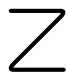
\includegraphics[keepaspectratio]{images/part002_15bf1a92.jpg}}

Remark. Note that two equivalent (H) functions can have non-equivalent inverses, as the example of the two functions \(\log x\) and \(1 + \log x\) shows.

\setcounter{exercisegroup}{0}
\refstepcounter{exercisegroup}
\section*{Exercises on \S\arabic{exercisegroup}}
\phantomsection
\addcontentsline{toc}{section}{Exercises on \protect\S\arabic{exercisegroup}}

\begin{enumerate}
\def\labelenumi{\arabic{enumi})}
\tightlist
\item
  Show that for \(x\) real tending to \(+\infty\) the function
\end{enumerate}

\[
f (x) = \left(x \cos^ {2} x + \sin^ {2} x\right) e ^ {x ^ {2}}
\]

is monotone, but is neither comparable to \(e^{x^2}\) nor weakly comparable to \(x^{1/2}e^{x^2}\) .

\begin{enumerate}
\def\labelenumi{\arabic{enumi})}
\setcounter{enumi}{1}
\tightlist
\item
  Let \(\varphi\) be a strictly positive function, defined and increasing for \(x > 0\) , and such that \(\varphi \gg 1\) .
\end{enumerate}

\begin{enumerate}
\def\labelenumi{\alph{enumi})}
\item
  Show that if the function \(\log \varphi(x) / \log x\) is increasing, then the relation \(f \ll g\) between functions \(>0\) implies that \(\varphi \circ f \ll \varphi \circ g\) if \(g \gg 1\) .
\item
  Give an example where \(\log \varphi(x)/\log x\) is decreasing, f and g are two functions \textgreater0 such that \(g \gg 1\) and \(f \sim g\) , but \(\varphi \circ f\) is not equivalent to \(\varphi \circ g\) .
\end{enumerate}

3) a) Let \((\alpha_{i},\beta_{i})\) be \(n\) distinct pairs of real numbers \(\geqslant 0\) , distinct from \((0,0)\) , and such that \(\inf_{i}\alpha_{i} = \inf_{i}\beta_{i} = 0\) . Consider the equation

\[
f (x, y) = \sum_ {i = 1} ^ {n} a _ {i} x ^ {\alpha_ {i}} y ^ {\beta_ {i}} \left(1 + \varphi_ {i} (x, y)\right) = 0
\]

where the \(a_{i}\) are real numbers \(\neq0\) and the \(\varphi_{i}\) are continuous functions on a square \(0\leqslant x\leqslant a,0\leqslant y\leqslant a\) , tending to 0 as \((x,y)\) tends to \((0,0)\) . Suppose that there exists a function g which is positive and continuous on an interval {[}0,b{]}, tending to 0 with x and such that \(f(x,g(x))=0\) for all \(x\in[0,b]\) . For every real number \(\mu>0\) show that \(g(x)/x^{\mu}\) tends to a limit, finite or infinite, as x tends to 0 (use V, p.~217, prop. 9, considering, for every number \(t\geqslant0\) , the equation \(f(x,tx^{\mu})=0\) ).

\begin{enumerate}
\def\labelenumi{\alph{enumi})}
\setcounter{enumi}{1}
\item
  For \(g(x)/x^{\mu}\) to tend to a finite limit \(\neq0\) it is necessary that \(\mu\) should be such that there exist at least two distinct pairs \((\alpha_{h},\beta_{h})\) and \((\alpha_{k},\beta_{k})\) such that \(\alpha_{h}+\mu\beta_{h}=\alpha_{k}+\mu\beta_{k}\) and such that, for every other pair \((\alpha_{i},\beta_{i})\) , one has \(\alpha_{i}+\mu\beta_{i}\geqslant\alpha_{h}+\mu\beta_{h}\) . One thus obtains a finite number of possible values \(\mu_{j}(1\leqslant j\leqslant r)\) ; the numbers \(-1/\mu_{j}\) are the gradients of the affine lines in the plane \(R^{2}\) which contain at least two of the set of points \((\alpha_{i},\beta_{i})\) and such that all the other points of this set lie above the line considered (``Newton polygon'').
\item
  Let \(\mu_{1}\) be the smallest of the numbers \(\mu_{j}\) . Show that \(g(x) / x^{\mu_1}\) tends to a finite limit (possibly zero). (Show first that one may always assume that if \(i\) and \(j\) are two distinct indices one cannot have both \(\alpha_{i} \leqslant \alpha_{j}\) and \(\beta_{i} \leqslant \beta_{j}\) ; deduce that one can assume \(\alpha_{1} = 0\) , \(\alpha_{i} > 0\) and \(\beta_{i} < \beta_{1}\) for \(i \neq 1\) ; now, putting \(g(x) = t(x)x^{\mu_1}\) , show that \(t(x)\) cannot tend to \(+\infty\) as \(x\) tends to 0.)
\end{enumerate}

\(d)\) Deduce from \(c\) ), by recursion on \(r\) , that there exists an index \(j\) such that \(g(x) / x^{\mu_j}\) tends to a finite limit \(\neq 0\) as \(x\) tends to 0.

\setcounter{exercisegroup}{2}
\refstepcounter{exercisegroup}
\section*{Exercises on \S\arabic{exercisegroup}}
\phantomsection
\addcontentsline{toc}{section}{Exercises on \protect\S\arabic{exercisegroup}}

\begin{enumerate}
\def\labelenumi{\arabic{enumi})}
\item
  Define an increasing function \(g\) , admitting a continuous derivative on a neighbourhood of \(+\infty\) , such that \(g\) and \(1 / x\) are comparable to order 1, but that \(x\) and \(1 / g\) are not comparable to order 1 (take \(g'(x) = 1\) except on sufficiently small intervals with centres at the points \(x = n\) ( \(n\) an integer \(>0\) ) on which \(g'\) takes very large values).
\item
  Let f and g be two functions \(\geqslant0\) tending to \(+\infty\) with x and comparable to order 1; if h is a differentiable function, \(\geqslant0\) and increasing as x tends to \(+\infty\) , show that hf and hg are comparable to order 1.
\item
  Give an example of two functions which are positive, decreasing, tend to 0 as x tends to \(+\infty\) , comparable to order 1 and such that \(xf(x)\) and \(xg(x)\) are not comparable to order 1 (take f and g equivalent and such that
\end{enumerate}

\[
\frac {f ^ {\prime} (x)}{f (x)} + \frac {1}{x} \qquad \text { and } \qquad \frac {g ^ {\prime} (x)}{g (x)} + \frac {1}{x}
\]

are not comparable).

\begin{enumerate}
\def\labelenumi{\arabic{enumi})}
\setcounter{enumi}{3}
\tightlist
\item
  \begin{enumerate}
  \def\labelenumii{\alph{enumii})}
  \tightlist
  \item
    Show that \(\frac{\sin x}{\sqrt{x}} \sim \frac{\sin x}{\sqrt{x}} \left(1 + \frac{\sin x}{\sqrt{x}}\right)\) , but that the integral \(\int_{a}^{+\infty} \frac{\sin t}{\sqrt{t}} dt\) converges while the integral \(\int_{a}^{+\infty} \frac{\sin t}{\sqrt{t}} \left(1 + \frac{\sin t}{\sqrt{t}}\right) dt\) is infinite.
  \end{enumerate}
\end{enumerate}

\begin{enumerate}
\def\labelenumi{\alph{enumi})}
\setcounter{enumi}{1}
\item
  Show that the integrals \(\int_{a}^{+\infty}\frac{\sin t}{t}dt\) and \(\int_{a}^{+\infty}\frac{\sin^{2}t}{t^{2}}dt\) are both convergent but that \(\int_{x}^{+\infty}\frac{\sin^{2}t}{t^{2}}dt\) is not negligible relative to \(\int_{x}^{+\infty}\frac{\sin t}{t}dt\) , even though \(\sin^{2}t/t^{2}\ll\sin t/t\) .
\item
  Consider the two continuous functions with values in \(R^{2}\) , defined on \([1, +\infty[\) :
\end{enumerate}

\[
\mathbf {f}: x \mapsto \left(\frac {1}{x ^ {2}}, \frac {\sin x}{x}\right), \quad \mathbf {g}: x \mapsto \left(\frac {1}{x ^ {2}}, \frac {\sin x}{x} \left(1 + \frac {\sin x}{x}\right)\right).
\]

Show that they do not vanish for any value of \(x\) , that \(\mathbf{f} \sim \mathbf{g}\) as \(x\) tends to \(+\infty\) , that the integrals \(\int_{a}^{+\infty} \mathbf{f}(t) dt\) and \(\int_{a}^{+\infty} \mathbf{g}(t) dt\) converge, but that \(\int_{x}^{+\infty} \mathbf{f}(t) dt\) is not equivalent to \(\int_{x}^{+\infty} \mathbf{g}(t) dt\) as \(x\) tends to \(+\infty\) .

5) Let \(f\) be a convex real function defined on a neighbourhood of \(+\infty\) such that \(f(x) \gg x\) . One says that \(f\) is regularly convex on a neighbourhood of \(+\infty\) if, for every convex function \(g\) defined on a neighbourhood of \(+\infty\) and such that \(f \sim g\) one also has \(f_d' \sim g_r'\) .

For every number \(\alpha > 0\) and x sufficiently large let \(k(\alpha, x)\) be the infimum of the numbers \(\left(f(y) - (y - x)f_{d}'(y)\right)/f(x)\) as y runs through the set of numbers \(\geqslant x\) such that \(f_{d}'(y) \leqslant (1 + \alpha)f_{d}'(x)\) . Similarly let \(h(\alpha, x)\) be the infimum of the numbers

\[
\left(f (z) + (x - z) f _ {d} ^ {\prime} (z)\right) / f (x)
\]

as \(z\) runs through the set of numbers \(\leqslant x\) such that \(f_d'(z) \geqslant (1 - \alpha)f_d'(x)\) . Let \(\psi(\alpha) = \limsup_{x \to +\infty} k(\alpha, x)\) , \(\varphi(\alpha) = \limsup_{x \to +\infty} h(\alpha, x)\) . Show that for \(f\) to be regularly convex on a

neighbourhood of \(+\infty\) it is necessary and sufficient that for all sufficiently small \(\alpha\) one has \(\psi(\alpha) < 1\) and \(\varphi(\alpha) < 1\) .

6) Let \(\mathbf{f}\) be a continuous vector function on an interval \([x_0, +\infty[\) of \(\mathbf{R}\) and such that for all \(\lambda \geqslant 0\) the function \(\mathbf{f}(x + \lambda) - \mathbf{f}(x)\) tends to 0 when \(x\) tends to \(+\infty\) .

\begin{enumerate}
\def\labelenumi{\alph{enumi})}
\tightlist
\item
  Show that \(\mathbf{f}(x+\lambda)-\mathbf{f}(x)\) tends uniformly to 0 with 1/x when \(\lambda\) belongs to any compact interval \(K=[a,b]\) of \([0,+\infty[\) . (Argue by contradiction: if there exists a sequence \((x_{n})\) tending to \(+\infty\) and a sequence of points \((\lambda_{n})\) of K such that
\end{enumerate}

\[
\| \mathbf {f} (x _ {n} + \lambda_ {n}) - \mathbf {f} (x _ {n}) \| > \alpha > 0
\]

for every n, then there exists a neighbourhood \(J_{n}\) of \(\lambda_{n}\) in K such that, for every \(\lambda \in J_{n}\) , one has \(\|\mathbf{f}(x_{n} + \lambda) - \mathbf{f}(x_{n})\| > \alpha\) . Construct by induction a decreasing sequence of closed intervals \(I_{k} \subset K\) and a subsequence \((x_{n_{k}})\) of \((x_{n})\) such that \(\|\mathbf{f}(x_{n_{k}} + \lambda) - \mathbf{f}(x_{n_{k}})\| \geqslant \alpha/3\) for every \(\lambda \in I_{k}\) ; remark for this that if \(\delta_{k}\) is the length of \(I_{k}\) and q an integer such that \(q\delta_{k} > b - a\) , then \(\|\mathbf{f}(x + \delta_{k}) - \mathbf{f}(x)\| \leqslant \alpha/3q\) once x is sufficiently large.)

\begin{enumerate}
\def\labelenumi{\alph{enumi})}
\setcounter{enumi}{1}
\tightlist
\item
  Deduce from \(a\) ) that \(\int_{x}^{x + 1}\mathbf{f}(t)dt - \mathbf{f}(x)\) tends to 0 as \(x\) tends to \(+\infty\) , and conclude that \(\mathbf{f}(x) = o(x)\) .
\end{enumerate}

\begin{enumerate}
\def\labelenumi{\arabic{enumi})}
\setcounter{enumi}{6}
\tightlist
\item
  Let g be a strictly positive real function, continuous on an interval \([x_{0}, +\infty[\) , and such that, for every \(\mu > 0\) , one has \(g(\mu x) \sim g(x)\) . Deduce from exerc. 6 that g is of order 0 relative to x.
\end{enumerate}

\setcounter{exercisegroup}{3}
\refstepcounter{exercisegroup}
\section*{Exercises on \S\arabic{exercisegroup}}
\phantomsection
\addcontentsline{toc}{section}{Exercises on \protect\S\arabic{exercisegroup}}

\begin{enumerate}
\def\labelenumi{\arabic{enumi})}
\item
  If the series with general term \(u_{n} \geqslant 0\) converges, so does the series with general term \(\sqrt{u_n u_{n+1}}\) . The converse is false in general; show that it holds if the series \((u_n)\) is decreasing.
\item
  Let \((p_{n})\) be an increasing sequence of numbers \textgreater{} 0 tending to \(+\infty\) .
\end{enumerate}

\begin{enumerate}
\def\labelenumi{\alph{enumi})}
\tightlist
\item
  If the ratio \(p_n / p_{n-1}\) tends to 1 as \(n\) increases indefinitely show that
\end{enumerate}

\[
\sum_ {k = 1} ^ {n} \frac {p _ {k} - p _ {k - 1}}{p _ {k}} \sim \log p _ {n}
\]

\[
\sum_ {k = 1} ^ {n} p _ {k} ^ {\rho} (p _ {k} - p _ {k - 1}) \sim \frac {1}{\rho + 1} p _ {n} ^ {\rho + 1} \quad \text { for } \rho > - 1
\]

(apply prop. 2 of V, p.~237).

\begin{enumerate}
\def\labelenumi{\alph{enumi})}
\setcounter{enumi}{1}
\item
  Without the hypothesis on the ratio \(p_{n}/p_{n-1}\) , show that the series with general term \((p_{n}-p_{n-1})/p_{n}\) always has an infinite sum (distinguish the two cases according to whether \(p_{n}/p_{n-1}\) tends to 1 or not).
\item
  Show that for every \(\rho > 0\) the series with general term \((p_n - p_{n-1}) / p_n p_{n-1}^\rho\) converges (compare to the series with general term \(\frac{1}{p_{n-1}^\rho} - \frac{1}{p_n^\rho}\) ).
\end{enumerate}

\begin{enumerate}
\def\labelenumi{\arabic{enumi})}
\setcounter{enumi}{2}
\item
  Show that, for every convergent series \((u_{n})\) with terms \(>0\) , there exists a series \((v_{n})\) with infinite sum, and terms \(>0\) , such that \(\liminf v_n / u_n = 0\) .
\item
  Let \((u_{n})\) be a decreasing sequence of numbers \textgreater0; if there exists an integer k such that \(ku_{kn} \geqslant u_{n}\) for all n from some point on, then the series with general term \(u_{n}\) has an infinite sum.
\item
  Let \((u_{n})\) be a series with terms \(>0\) from some point on. Show that if
\end{enumerate}

\[
\operatorname * {l i m s u p} _ {n \to \infty} \left(\frac {u _ {n + 1}}{u _ {n}}\right) ^ {n} <   \frac {1}{e}
\]

then the series converges, and if \(\liminf_{n\to\infty}\left(\frac{u_{n+1}}{u_n}\right)^n\geqslant\frac{1}{e}\) the series has an infinite sum.

\begin{enumerate}
\def\labelenumi{\arabic{enumi})}
\setcounter{enumi}{5}
\item
  Let \((u_{n})\) be a series of reals \(\neq 0\) such that \(\lim_{n\to \infty}u_n = 0\) . Show that if there exists a number \(r\) such that \(0 < r < 1\) and if from some point on one has \(-1\leqslant u_{n + 1} / u_n\leqslant r\) , then the series \((u_{n})\) converges.
\item
  Let \((u_{n})\) be a convergent series with terms \(>0\) .
\end{enumerate}

\begin{enumerate}
\def\labelenumi{\alph{enumi})}
\tightlist
\item
  Show that
\end{enumerate}

\[
\lim _ {n \rightarrow \infty} \frac {u _ {1} + 2 u _ {2} + \cdots + n u _ {n}}{n} = 0.
\]

\begin{enumerate}
\def\labelenumi{\alph{enumi})}
\setcounter{enumi}{1}
\tightlist
\item
  Show that
\end{enumerate}

\[
\sum_ {n = 1} ^ {\infty} \frac {u _ {1} + 2 u _ {2} + \cdots + n u _ {n}}{n (n + 1)} = \sum_ {n = 1} ^ {\infty} u _ {n}
\]

\[
\left(\text { write } \frac {1}{n (n + 1)} = \frac {1}{n} - \frac {1}{n + 1}\right).
\]

\begin{enumerate}
\def\labelenumi{\alph{enumi})}
\setcounter{enumi}{2}
\tightlist
\item
  Deduce from a) and b) that
\end{enumerate}

\[
\lim _ {n \to \infty} n (u _ {1} u _ {2} \dots u _ {n}) ^ {1 / n} = 0
\]

and that

\[
\sum_ {n = 1} ^ {\infty} \frac {(n ! u _ {1} u _ {2} \dots u _ {n}) ^ {1 / n}}{n + 1} <   \sum_ {n = 1} ^ {\infty} u _ {n}
\]

(apply the inequality (8) of III, p.~93).

8) a) Let \((z_{n})\) be a sequence of complex numbers. Show that if the series with general terms \(z_{n}, z_{n}^{2}, \ldots, z_{n}^{q-1}, |z_{n}|^{q}\) converge, then the infinite product with general factor \(1 + z_{n}\) converges.

\begin{enumerate}
\def\labelenumi{\alph{enumi})}
\setcounter{enumi}{1}
\tightlist
\item
  If \(z_{n}\) is real and if the series with general term \(z_{n}\) converges, then the infinite product with general factor \(1 + z_{n}\) converges if the series with general term \(z_{n}^{2}\) converges, and one has
\end{enumerate}

\[
\underset {n = 1} {\overset {\infty} {\mathrm{P}}} (1 + z _ {n}) = 0 \quad \text { if } \quad \sum_ {n = 1} ^ {\infty} z _ {n} ^ {2} = + \infty .
\]

\begin{enumerate}
\def\labelenumi{\alph{enumi})}
\setcounter{enumi}{2}
\tightlist
\item
  For every integer \(p \geqslant 2\) put
\end{enumerate}

\[
k _ {p} = [ \log \log p ], \quad h _ {p} = \sum_ {j = 1} ^ {p - 1} k _ {j}, \quad \omega_ {p} = \frac {2 \pi}{k _ {p}}.
\]

Define the sequence \((z_{n})\) of complex numbers in the following way: for \(n = h_{p} + m\) , \(0 \leqslant m \leqslant k_{p} - 1\) , put \(z_{n} = e^{mi\omega_{p}} / \log p\) . Show that for every integer q \textgreater{} 0 the series with general term \(z_{n}^{q}\) converges, but that the product with general factor \(1 + z_{n}\) does not converge.

\begin{enumerate}
\def\labelenumi{\arabic{enumi})}
\setcounter{enumi}{8}
\tightlist
\item
  \begin{enumerate}
  \def\labelenumii{\alph{enumii})}
  \tightlist
  \item
    Show, with the help of Stirling's formula, that the maximum of the function \(f_{n}(x) = \left|e^{-2x} - e^{-x}\sum_{k=0}^{n}(-1)^{k}\frac{x^{k}}{k!}\right|\) over the interval \([0, +\infty[\) tends to 0 with \(1/n\) .
  \end{enumerate}
\end{enumerate}

\begin{enumerate}
\def\labelenumi{\alph{enumi})}
\setcounter{enumi}{1}
\tightlist
\item
  Deduce, by induction on the integer p, that for every \(\varepsilon > 0\) there exists a polynomial \(g(x)\) such that \(\left|e^{-px} - e^{-x}g(x)\right| \leqslant \varepsilon\) for every \(x \geqslant 0\) (replace x by px/2 in a), and apply the induction hypothesis to \(e^{-(p-1)x/2}\) .
\end{enumerate}

\begin{enumerate}
\def\labelenumi{\arabic{enumi})}
\setcounter{enumi}{9}
\tightlist
\item
  For every number \(\alpha > 0\) derive the formula
\end{enumerate}

\[
1 ^ {\alpha n} + 2 ^ {\alpha n} + \dots + n ^ {\alpha n} \sim \frac {n ^ {\alpha n}}{1 - e ^ {- \alpha}}
\]

as n tends to \(+\infty\) .

11) For every number \(\alpha > 0\) derive the formula

\[
(1!) ^ {- \alpha / n} + (2!) ^ {- \alpha / n} + \dots + (n!) ^ {- \alpha / n} \sim \frac {1}{\alpha} \frac {n}{\log n}
\]

as \(n\) tends to \(+\infty\) (compare each term \((p!)^{-\alpha / n}\) to \(n^{-\alpha p / n}\) ).

\section*{Exercises on the Appendix}
\phantomsection
\addcontentsline{toc}{section}{Exercises on the Appendix}

\begin{enumerate}
\def\labelenumi{\arabic{enumi})}
\tightlist
\item
  Let \(\mathfrak{K}\) be a Hardy field such that, for every function \(f\in \mathfrak{K}\) not identically zero on a neighbourhood of \(+\infty\) there exists a \(\lambda >0\) such that
\end{enumerate}

\[
\frac {1}{e _ {m} (x ^ {\lambda})} \ll f (x) \ll e _ {m} (x ^ {\lambda})
\]

(m an integer independent of f).

\begin{enumerate}
\def\labelenumi{\alph{enumi})}
\tightlist
\item
  Let \(u_{1}, u_{2}, \ldots, u_{p}\) be p functions of the form \(u_{k} = \log |z_{k}|\) , where \(z_{k} \in K\) is not zero on a neighbourhood of \(+\infty\) . Show that for every function g (not zero on a neighbourhood of \(+\infty\) ) of the Hardy field \(\mathfrak{K}(u_{1}, u_{2}, \ldots, u_{p})\) obtained by adjoining the functions \(u_{k}\) ( \(1 \leqslant k \leqslant p\) ) to K, there exists a number \(\mu > 0\) such that
\end{enumerate}

\[
\frac {1}{e _ {m} (x ^ {\mu})} \ll g (x) \ll e _ {m} (x ^ {\mu})
\]

(reduce to the case where g is a polynomial in the \(u_{k}\) with coefficients in K and argue by induction on p, then, for p = 1, argue by induction on the degree of the polynomial g, proceeding as in lemma 2 of V, p.~248).

\begin{enumerate}
\def\labelenumi{\alph{enumi})}
\setcounter{enumi}{1}
\tightlist
\item
  Let \(u_{k}\) ( \(1 \leqslant k \leqslant p\) ) be \(p\) functions of the form \(u_{k} = \exp(z_{k})\) where \(z_{k} \in \mathcal{K}\) . Show that for every function \(g\) of the Hardy field \(\mathcal{K}(u_{1}, u_{2}, \ldots, u_{p})\) not identically zero on a neighbourhood of \(+\infty\) there exists a number \(\mu > 0\) such that
\end{enumerate}

\[
\frac {1}{e _ {m + 1} (x ^ {\mu})} \prec g (x) \prec e _ {m + 1} (x ^ {\mu})
\]

(similar method).

\begin{enumerate}
\def\labelenumi{\alph{enumi})}
\setcounter{enumi}{2}
\tightlist
\item
  Deduce that if \(f\) is an (H) function having a definition sequence with \(n\) terms, and not identically zero on a neighbourhood of \(+\infty\) , there exists a number \(\lambda > 0\) such that
\end{enumerate}

\[
\frac {1}{e _ {n} (x ^ {\lambda})} \ll f (x) \ll e _ {n} (x ^ {\lambda}).
\]

\begin{enumerate}
\def\labelenumi{\arabic{enumi})}
\setcounter{enumi}{1}
\tightlist
\item
  \begin{enumerate}
  \def\labelenumii{\alph{enumii})}
  \tightlist
  \item
    Show that every (H) function having a definition sequence of just one term is equivalent to a function of one of the forms \(x^{p}(\log x)^{q}\) , or \(x^{p}e^{g(x)}\) , where p and q are rational integers and g is a polynomial in x (method of exerc. 1).
  \end{enumerate}
\end{enumerate}

\begin{enumerate}
\def\labelenumi{\alph{enumi})}
\setcounter{enumi}{1}
\tightlist
\item
  Deduce from a) that every function in the Hardy field \(\mathbf{R}(x,u_{1},\ldots,u_{p})\) , where \(u_{1},\ldots,u_{p}\) are (H) functions having a single-term definition sequence, is equivalent to a function of the form \(x^{p}(\log x)^{q}e^{g(x)}\) where p and q are rational integers and g is a polynomial in x.
\end{enumerate}

\begin{enumerate}
\def\labelenumi{\arabic{enumi})}
\setcounter{enumi}{2}
\item
  Let f and g be two (H) functions such that f/g is of order 0 relative to \(l_{m}(x)\) ; show that if g is not of order 0 relative to \(l_{m}(x)\) one has \(f'/g' \sim f/g\) (compare \(\log |f|\) and \(\log |g|\) ).
\item
  Let \(\mathfrak{K}\) be a Hardy field such that, for every function \(f\in \mathfrak{K}\) not equivalent to a constant, and of order 0 relative to \(l_{m - 1}(x)\) , there exist a constant \(k\) and a rational integer \(r\) such that \(f(x)\sim k(l_m(x))^r\) .
\end{enumerate}

\begin{enumerate}
\def\labelenumi{\alph{enumi})}
\item
  Let z be any function in K, not identically zero on a neighbourhood of \(+\infty\) . Show that every function g in the Hardy field \(\mathcal{K}(\log|z|)\) not equivalent to a constant, and of order 0 relative to \(l_{m}(x)\) , is equivalent to a function of the form \(k(l_{m+1}(x))^{r}\) (k constant, r a rational integer). (First consider the case where g is a polynomial of degree p in \(\log|z|\) , with coefficients in K, and argue by induction on p, using exerc. 3; if g is a rational function of \(\log|z|\) , with coefficients in K, argue by induction on the degree of the numerator, using exerc. 3.)
\item
  Show that every function in \(\mathfrak{K}(l_{m+1}(x))\) is equivalent to a function of the form \(f(x)(l_{m+1}(x))^r\) where \(f \in \mathfrak{K}\) and \(r\) is a rational integer.
\item
  Let z be any function in K. Show that every function g of the Hardy field \(\mathfrak{K}(e^{z})\) of order 0 relative to \(l_{m}(x)\) is equivalent to a constant. (First consider the case where \(g = u^{q} \mathrm{P}(u)\) , where \(u = e^{z}\) , q is a rational integer, and \(\mathrm{P}(u)\) is a polynomial in u, of degree p, with coefficients in K; then argue by induction on p, using a) and exerc. 3. Pass from there to the general case by using exerc. 3.)
\item
  Extend the result of a) to the field \(\mathfrak{K}(u_{1}, u_{2}, \ldots, u_{s})\) , where the \(u_{k}\) are of the form \(e^{z_{k}}\) or \(\log |z_{k}|\) , the \(z_{k}\) being functions in K not identically zero on a neighbourhood of \(+\infty\) (argue by induction on s).
\end{enumerate}

\begin{enumerate}
\def\labelenumi{\arabic{enumi})}
\setcounter{enumi}{4}
\tightlist
\item
  \begin{enumerate}
  \def\labelenumii{\alph{enumii})}
  \tightlist
  \item
    Deduce from exerc. 4 that if f is an (H) function having a definition sequence of n terms, not equivalent to a constant, and of order 0 relative to \(l_{n-1}(x)\) , there exist a constant k and a rational integer r such that \(f(x) \sim k(l_n(x))^r\) .
  \end{enumerate}
\end{enumerate}

\begin{enumerate}
\def\labelenumi{\alph{enumi})}
\setcounter{enumi}{1}
\tightlist
\item
  Deduce from exerc. 4 that if \(f\) is any (H) function there exists an integer \(n\) such that the logarithmic criterion of order \(n\) will determine whether the integral \(\int_{a}^{+\infty} f(t) dt\) converges or is infinite.
\end{enumerate}

\begin{enumerate}
\def\labelenumi{\arabic{enumi})}
\setcounter{enumi}{5}
\tightlist
\item
  Compare among themselves the functions \(e_p\left((l_q(x))^{\mu}\right)\) according to the values of the integers \(p\) and \(q\) and the real number \(\mu\) , assumed \(> 0\) and \(\neq 1\) .
\end{enumerate}

7) Let \(f\) be an (H) function having a definition sequence of \(n\) terms. Show that if one has \(e_p((l_{q+1}(x))^{\beta}) \ll f(x) \ll e_p((l_q(x))^{\alpha})\) (resp. \(e_p((l_q(x))^{\beta}) \ll f(x) \ll e_{p+1}((l_q(x))^{\alpha}))\) )

for every \(\beta > 0\) and every \(\alpha\) such that \(0 < \alpha < 1\) , then necessarily \(p + q + 1 < n\) (argue by induction on \(n\) , using methods similar to those of exerc. 1 (V, p.~263) and 4 (V, p.~264)).

\begin{enumerate}
\def\labelenumi{\arabic{enumi})}
\setcounter{enumi}{7}
\tightlist
\item
  \begin{enumerate}
  \def\labelenumii{\alph{enumii})}
  \tightlist
  \item
    Let \((f_{n})\) be a sequence of increasing continuous functions belonging to \(\mathcal{H}(\mathfrak{F},\mathbf{R})\) and such that \(f_{n} \ll f_{n+1}\) for every n.~Show that there exists a function f that is continuous, increasing, belongs to \(\mathcal{H}(\mathfrak{F},\mathbf{R})\) , and is such that \(f \gg f_{n}\) for every n (reduce to the case where \(f_{n} \leqslant f_{n+1}\) and define f so that \(f_{n}(x) \leqslant f(x) \leqslant f_{n+1}(x)\) for \(n \leqslant x \leqslant n+1\) ).
  \end{enumerate}
\end{enumerate}

\begin{enumerate}
\def\labelenumi{\alph{enumi})}
\setcounter{enumi}{1}
\item
  Let \((f_n)\) be a sequence of increasing continuous functions belonging to \(\mathcal{H}(\mathfrak{F},\mathbf{R})\) and such that \(1\ll f_{n + 1}\ll f_n\) for every \(n\) . Show that there exists a function \(f\) that is continuous, increasing, belongs to \(\mathcal{H}(\mathfrak{F},\mathbf{R})\) , and is such that \(1\ll f\ll f_n\) for every \(n\) (reduce to the case where \(f_{n + 1}\leqslant f_n\) and show that one can define an increasing sequence \((x_{n})\) of real numbers and a continuous increasing function \(f\) such that \(f_{n + 1}(x)\leqslant f(x)\leqslant f_n(x)\) for \(x_{n}\leqslant x\leqslant x_{n + 1}\) ).
\item
  Let \((f_n), (g_n)\) be two sequences of continuous increasing functions belonging to \(\mathcal{H}(\mathfrak{F}, \mathbf{R})\) such that \(f_n \ll f_{n+1}\) , \(g_m \gg g_{m+1}\) and \(f_n \ll g_m\) for all \(m\) and \(n\) ; show that there exists a function \(h\) , continuous, increasing, belonging to \(\mathcal{H}(\mathfrak{F}, \mathbf{R})\) , such that \(f_n \ll h \ll g_m\) for all \(m\) and \(n\) (similar method).
\end{enumerate}

In particular, show that there exists a continuous decreasing function \(f\) in \(\mathcal{H}(\mathfrak{F},\mathbf{R})\) such that no logarithmic criterion allows one to determine whether the integral \(\int_{a}^{+\infty}f(t)dt\) converges or is infinite (``theorems of Du Bois-Reymond'').

\begin{enumerate}
\def\labelenumi{\arabic{enumi})}
\setcounter{enumi}{8}
\item
  Show that the series \(\sum_{n=1}^{\infty} \frac{e_n(x)}{e_n(n)}\) converges uniformly on every compact subset of \(\mathbf{R}\) , and that its sum \(f(x)\) is such that \(f(x) \gg e_n(x)\) for every integer \(n\) .
\item
  Show that there exists an increasing function \(f\) , defined, continuous and \(> 0\) for \(x \geqslant 0\) , such that \(f(2x) = 2^{f(x)}\) for all \(x \geqslant 0\) ; deduce from this that \(f(x) \gg e_n(x)\) for every integer \(n\) .
\item
  Let \(f\) be an increasing function, continuous and \(\geqslant 0\) , defined for \(x \geqslant 0\) , and such that \(f(x) \gg e_n(x)\) for every integer \(n\) ; show that, if \(g\) is the inverse function of \(f\) , one has \(1 \ll g(x) \ll l_n(x)\) for every integer \(n\) .
\end{enumerate}

12) For every integer \(n > 0\) let \(n = \sum_{k=0}^{\infty} \varepsilon_k 2^k\) be the dyadic expansion of \(n\) ( \(\varepsilon_k\) is an integer, zero for all but a finite number of indices, \(0 \leqslant \varepsilon_k \leqslant 1\) ). Put

\[
\alpha (n) = \sum_ {k = 0} ^ {\infty} \varepsilon_ {k}, \quad \mathrm{A} _ {1} (n) = \sum_ {j = 1} ^ {n} \alpha (j), \quad \mathrm{A} _ {2} (n) = \sum_ {j = 1} ^ {n} \alpha (\alpha (j)).
\]

\begin{enumerate}
\def\labelenumi{\alph{enumi})}
\tightlist
\item
  Prove the formula \(\mathrm{A}_1(n) = \sum_{k=0}^{\infty}(k+2)\varepsilon_k 2^{k-1}\) . Deduce the formula
\end{enumerate}

\[
\mathrm{A} _ {1} (n) = \frac {n}{2} \frac {\log n}{\log 2} + o (n \log \log n)
\]

as \(n\) grows indefinitely (decompose the sum which expresses \(\mathrm{A}_1(n)\) into two parts, the index \(k\) varying from 0 to \(\mu(n)\) in the first sum, from \(\mu(n)\) to \(n_1\) in the second, where \(n_1\) is the largest of the numbers \(k\) such that \(\varepsilon_k \neq 0\) and \(\mu(n)\) is chosen suitably; bound the first sum using prop. 6 of V, p.~239, and then estimate the difference between the second sum and \(n_1n / 2\) .

\begin{enumerate}
\def\labelenumi{\alph{enumi})}
\setcounter{enumi}{1}
\tightlist
\item
  Establish the relation
\end{enumerate}

\[
\sum_ {j = 0} ^ {2 ^ {m} - 1} f (\alpha (j)) = \sum_ {k = 0} ^ {m} \binom {m} {k} f (k)
\]

\(f\) being an arbitrary function defined on \(\mathbf{N}\) (for a given \(k\) consider the number of \(j < 2^{m}\) such that \(\alpha(j) = k\) ).

\begin{enumerate}
\def\labelenumi{\alph{enumi})}
\setcounter{enumi}{2}
\tightlist
\item
  For \(m = 2^r - 1\) show that \(\alpha(m - j) + \alpha(j) = r\) . Deduce from this and from \(b\) ) that
\end{enumerate}

\[
\mathrm{A} _ {2} (2 ^ {m}) = r 2 ^ {m - 1} \sim \frac {2 ^ {m} \log \log 2 ^ {m}}{2 \log 2}.
\]

\begin{enumerate}
\def\labelenumi{\alph{enumi})}
\setcounter{enumi}{3}
\tightlist
\item
  For \(m = 2^{r}\) show that
\end{enumerate}

\[
\mathrm{A} _ {2} (2 ^ {m}) = 2 \mathrm{A} _ {2} (2 ^ {m - 1}) + 2 ^ {m - 1} - \sum_ {j = 0} ^ {m - 1} \binom {m - 1} {j} \Delta (j + 1)
\]

where we have put \(\alpha(n+1)-\alpha(n)=1-\Delta(n+1)\) for all \(n\) (use \(b\) ) and the relation \(\alpha(2^{k}+r)=\alpha(r)+1\) for \(r<2^{k}\) ). Show that \(\sum_{j=0}^{m-1}\binom{m-1}{j}\Delta(j+1)\leqslant r^{m-2}\) (remark that \(\Delta(j+1)=0\) if \(j\) is even, and \(\Delta(j+1)\leqslant\log j/\log 2\) for all \(j\) ). Deduce, with the help of \(c\) ), that

\[
\mathrm{A} _ {2} (2 ^ {m}) \geqslant \frac {3}{2} r 2 ^ {m - 1} \geqslant \frac {3}{2} \frac {2 ^ {m} \log \log 2 ^ {m}}{2 \log 2}.
\]

Conclude from \(c\) ) and this relation that \(\mathrm{A}_2(n)\) is not equivalent to any (H) function as \(n\) tends to \(+\infty\) .

\begin{enumerate}
\def\labelenumi{\arabic{enumi})}
\setcounter{enumi}{12}
\tightlist
\item
  Let \(f\) be an (H) function such that \(1 \prec f(x) \prec x\) . Show that in the Taylor formula
\end{enumerate}

\[
\begin{array}{l} f (x + f (x)) = f (x) + f (x) f ^ {\prime} (x) + \frac {1}{2 !} (f (x)) ^ {2} f ^ {\prime \prime} (x) + \dots + \\ \qquad + \frac {1}{n !} (f (x)) ^ {n} f ^ {(n)} (x) + \frac {1}{(n + 1) !} (f (x)) ^ {n + 1} f ^ {(n + 1)} (x + \theta f (x)) \end{array}
\]

with \(0 < \theta < 1\) (I, p.~42, exerc. 9) each term is negligible relative to the previous one. If f is of order \textless{} 1 relative to x, the last term in this sum tends to 0 with 1/x once n is sufficiently large.

\begin{enumerate}
\def\labelenumi{\arabic{enumi})}
\setcounter{enumi}{13}
\tightlist
\item
  Deduce from exerc. 13 that if \(f\) is an (H) function such that \(\log f(e^x)\) is of order \(< 1\) relative to \(x\) , the function \(f(xf(x))\) is equivalent to a function of the form \(e^{g(x)}\) , where \(g\) is a rational function of \(x\) , \(\log f(x)\) , and of a certain number of derivatives of this last function.
\end{enumerate}

15) Let \(f\) be an (H) function, convex on a neighbourhood of \(+\infty\) , such that \(f(x) \gg x\) . For every \(\alpha > 0\) let \(x_{\alpha}\) be the point such that \(f'(x_{\alpha}) = (1 + \alpha)f'(x)\) .

\begin{enumerate}
\def\labelenumi{\alph{enumi})}
\tightlist
\item
  If \(f\) is of order \(+\infty\) relative to \(x\) show that
\end{enumerate}

\[
x _ {\alpha} - x \sim \log (1 + \alpha) \frac {f (x)}{f ^ {\prime} (x)}
\]

(use prop. 2 (V, p.~251) and 4 (V, p.~255), applying the Taylor formula to \(\log f'(x)\) ). Show that \(\left(f(x_{\alpha}) - (x_{\alpha} - x)f'(x_{\alpha})\right)/f(x)\) tends to \((1 + \alpha)\left(1 - \log(1 + \alpha)\right)\) as \(x\) tends to \(+\infty\) .

\begin{enumerate}
\def\labelenumi{\alph{enumi})}
\setcounter{enumi}{1}
\tightlist
\item
  If \(f\) is of order \(r > 1\) relative to \(x\) show that
\end{enumerate}

\[
x _ {\alpha} \sim (1 + \alpha) ^ {1 / (r - 1)} x
\]

(remark that if \(f_{1}\) is of order 0 relative to \(x\) one has \(f_{1}(kx) \sim f_{1}(x)\) for every constant \(k\) , by prop. 4 of V, p.~255). Deduce that \(\left(f(x_{\alpha}) - (x_{\alpha} - x)f'(x_{\alpha})\right) / f(x)\) tends to

\[
r (1 + \alpha) - (r - 1) (1 + \alpha) ^ {r / (r - 1)}
\]

as \(x\) tends to \(+\infty\) .

\begin{enumerate}
\def\labelenumi{\alph{enumi})}
\setcounter{enumi}{2}
\tightlist
\item
  Suppose finally that \(f\) is of order 1 relative to \(x\) . Putting \(f(x) = xf_1(x)\) show that
\end{enumerate}

\[
x _ {\alpha} - x \sim \log (1 + \alpha) \frac {f _ {1} (x)}{f _ {1} ^ {\prime} (x)}
\]

(consider the inverse function of \(f_{1}\) , which is of order \(+\infty\) relative to \(x\) ). Deduce that \(\left(f(x_{\alpha}) - (x_{\alpha} - x)f'(x_{\alpha})\right) / f(x)\) tends to \(-\infty\) as \(x\) tends to \(+\infty\) .

Similarly let \(x_{\alpha}'\) be the point such that \(f'(x_{\alpha}') = (1 - \alpha)f'(x)\) (for \(0 < \alpha < 1\) ). State the formulae analogous to the previous ones that express the principal part of \(x - x_{\alpha}'\) and the limit of

\[
\left(f (x _ {\alpha} ^ {\prime}) + (x - x _ {\alpha} ^ {\prime}) f ^ {\prime} (x _ {\alpha} ^ {\prime})\right) / f (x)
\]

as \(x\) tends to \(+\infty\) .

Conclude from these results that \(f\) is a regularly convex function on a neighbourhood of \(+\infty\) (V, p.~260, exerc. 5).

\makeatletter
\gdef\@chapapp{\chaptername}
\makeatother
\renewcommand{\thechapter}{\Roman{chapter}}
\renewcommand{\thesection}{\S\arabic{section}}
\setcounter{chapter}{5}
\chapter{Generalized Taylor expansions: Euler-Maclaurin summation formula}

\section{GENERALIZED TAYLOR EXPANSIONS}
